% Template for PLoS
% Version 3.5 March 2018
%
% % % % % % % % % % % % % % % % % % % % % %
%
% -- IMPORTANT NOTE
%
% This template contains comments intended 
% to minimize problems and delays during our production 
% process. Please follow the template instructions
% whenever possible.
%
% % % % % % % % % % % % % % % % % % % % % % % 
%
% Once your paper is accepted for publication, 
% PLEASE REMOVE ALL TRACKED CHANGES in this file 
% and leave only the final text of your manuscript. 
% PLOS recommends the use of latexdiff to track changes during review, as this will help to maintain a clean tex file.
% Visit https://www.ctan.org/pkg/latexdiff?lang=en for info or contact us at latex@plos.org.
%
%
% There are no restrictions on package use within the LaTeX files except that 
% no packages listed in the template may be deleted.
%
% Please do not include colors or graphics in the text.
%
% The manuscript LaTeX source should be contained within a single file (do not use \input, \externaldocument, or similar commands).
%
% % % % % % % % % % % % % % % % % % % % % % %
%
% -- FIGURES AND TABLES
%
% Please include tables/figure captions directly after the paragraph where they are first cited in the text.
%
% DO NOT INCLUDE GRAPHICS IN YOUR MANUSCRIPT
% - Figures should be uploaded separately from your manuscript file. 
% - Figures generated using LaTeX should be extracted and removed from the PDF before submission. 
% - Figures containing multiple panels/subfigures must be combined into one image file before submission.
% For figure citations, please use "Fig" instead of "Figure".
% See http://journals.plos.org/plosone/s/figures for PLOS figure guidelines.
%
% Tables should be cell-based and may not contain:
% - spacing/line breaks within cells to alter layout or alignment
% - do not nest tabular environments (no tabular environments within tabular environments)
% - no graphics or colored text (cell background color/shading OK)
% See http://journals.plos.org/plosone/s/tables for table guidelines.
%
% For tables that exceed the width of the text column, use the adjustwidth environment as illustrated in the example table in text below.
%
% % % % % % % % % % % % % % % % % % % % % % % %
%
% -- EQUATIONS, MATH SYMBOLS, SUBSCRIPTS, AND SUPERSCRIPTS
%
% IMPORTANT
% Below are a few tips to help format your equations and other special characters according to our specifications. For more tips to help reduce the possibility of formatting errors during conversion, please see our LaTeX guidelines at http://journals.plos.org/plosone/s/latex
%
% For inline equations, please be sure to include all portions of an equation in the math environment.  For example, x$^2$ is incorrect; this should be formatted as $x^2$ (or $\mathrm{x}^2$ if the romanized font is desired).
%
% Do not include text that is not math in the math environment. For example, CO2 should be written as CO\textsubscript{2} instead of CO$_2$.
%
% Please add line breaks to long display equations when possible in order to fit size of the column. 
%
% For inline equations, please do not include punctuation (commas, etc) within the math environment unless this is part of the equation.
%
% When adding superscript or subscripts outside of brackets/braces, please group using {}.  For example, change "[U(D,E,\gamma)]^2" to "{[U(D,E,\gamma)]}^2". 
%
% Do not use \cal for caligraphic font.  Instead, use \mathcal{}
%
% % % % % % % % % % % % % % % % % % % % % % % % 
%
% Please contact latex@plos.org with any questions.
%
% % % % % % % % % % % % % % % % % % % % % % % %

\documentclass[10pt,letterpaper]{article}
\usepackage[top=0.85in,left=2.75in,footskip=0.75in]{geometry}

% amsmath and amssymb packages, useful for mathematical formulas and symbols
\usepackage{amsmath,amssymb}

% Use adjustwidth environment to exceed column width (see example table in text)
\usepackage{changepage}

% Use Unicode characters when possible
\usepackage[utf8x]{inputenc}

% textcomp package and marvosym package for additional characters
\usepackage{textcomp,marvosym}

% cite package, to clean up citations in the main text. Do not remove.
\usepackage{cite}

% Use nameref to cite supporting information files (see Supporting Information section for more info)
\usepackage{nameref,hyperref}

% line numbers
\usepackage[right]{lineno}

% ligatures disabled
\usepackage{microtype}
\DisableLigatures[f]{encoding = *, family = * }

% color can be used to apply background shading to table cells only
\usepackage[table]{xcolor}

% array package and thick rules for tables
\usepackage{array}

% create "+" rule type for thick vertical lines
\newcolumntype{+}{!{\vrule width 2pt}}

% create \thickcline for thick horizontal lines of variable length
\newlength\savedwidth
\newcommand\thickcline[1]{%
  \noalign{\global\savedwidth\arrayrulewidth\global\arrayrulewidth 2pt}%
  \cline{#1}%
  \noalign{\vskip\arrayrulewidth}%
  \noalign{\global\arrayrulewidth\savedwidth}%
}

% \thickhline command for thick horizontal lines that span the table
\newcommand\thickhline{\noalign{\global\savedwidth\arrayrulewidth\global\arrayrulewidth 2pt}%
\hline
\noalign{\global\arrayrulewidth\savedwidth}}


% Remove comment for double spacing
%\usepackage{setspace} 
%\doublespacing

% Text layout
\raggedright
\setlength{\parindent}{0.5cm}
\textwidth 5.25in 
\textheight 8.75in

% Bold the 'Figure #' in the caption and separate it from the title/caption with a period
% Captions will be left justified
\usepackage[aboveskip=1pt,labelfont=bf,labelsep=period,justification=raggedright,singlelinecheck=off]{caption}
\renewcommand{\figurename}{Fig}

% Use the PLoS provided BiBTeX style
\bibliographystyle{plos2015}

% Remove brackets from numbering in List of References
\makeatletter
\renewcommand{\@biblabel}[1]{\quad#1.}
\makeatother



% Header and Footer with logo
\usepackage{lastpage,fancyhdr,graphicx}
\usepackage{epstopdf}
%\pagestyle{myheadings}
\pagestyle{fancy}
\fancyhf{}
%\setlength{\headheight}{27.023pt}
%\lhead{
\includegraphics[width=2.0in]{PLOS-submission.eps}}
\rfoot{\thepage/\pageref{LastPage}}
\renewcommand{\headrulewidth}{0pt}
\renewcommand{\footrule}{\hrule height 2pt \vspace{2mm}}
\fancyheadoffset[L]{2.25in}
\fancyfootoffset[L]{2.25in}
\lfoot{\today}

%% Include all macros below

\newcommand{\lorem}{{\bf LOREM}}
\newcommand{\ipsum}{{\bf IPSUM}}

%% END MACROS SECTION

\newcommand{\grace}[1]{\textcolor{blue}{#1}}
\newcommand{\ruchi}[1]{\textcolor{red}{#1}}
\newcommand{\sticky}{proglobular~}
\usepackage{makecell}

\renewcommand\theadalign{bc}
\renewcommand\theadfont{\bfseries}
\renewcommand\theadgape{\Gape[4pt]}
\renewcommand\cellgape{\Gape[4pt]}


\begin{document}
\vspace*{0.2in}

% Title must be 250 characters or less.
\begin{flushleft}
{\Large
\textbf\newline{Sequence specificity despite intrinsic disorder: how a disease-associated Val/Met polymorphism rearranges tertiary interactions in a long disordered protein} % Please use "sentence case" for title and headings (capitalize only the first word in a title (or heading), the first word in a subtitle (or subheading), and any proper nouns).
}
\newline
% Insert author names, affiliations and corresponding author email (do not include titles, positions, or degrees).
\\
Ruchi Lohia\textsuperscript{1},
Reza Salari\textsuperscript{1},
Grace Brannigan\textsuperscript{1,2*},
\\
\bigskip
\textbf{1} Center for Computational and Integrative Biology, Rutgers University, Camden, NJ, USA
\\
\textbf{2} Department of Physics, Rutgers University, Camden, NJ, USA
\\
\bigskip

% Insert additional author notes using the symbols described below. Insert symbol callouts after author names as necessary.
% 
% Remove or comment out the author notes below if they aren't used.
%
% Primary Equal Contribution Note
%\Yinyang These authors contributed equally to this work.

% Additional Equal Contribution Note
% Also use this double-dagger symbol for special authorship notes, such as senior authorship.
%\ddag These authors also contributed equally to this work.

% Current address notes
%\textcurrency Current Address: Dept/Program/Center, Institution Name, City, State, Country % change symbol to "\textcurrency a" if more than one current address note
% \textcurrency b Insert second current address 
% \textcurrency c Insert third current address

% Deceased author note
%\dag Deceased

% Group/Consortium Author Note
%\textpilcrow Membership list can be found in the Acknowledgments section.

% Use the asterisk to denote corresponding authorship and provide email address in note below.
* grace.brannigan@rutgers.edu(GB)

\end{flushleft}

\renewcommand{\thepage}{S\arabic{page}}  
\renewcommand{\thesection}{S\arabic{section}}   
\renewcommand{\thetable}{S\arabic{table}}   
\renewcommand{\figurename}{}
\renewcommand{\thefigure}{S\arabic{figure} Fig}

\clearpage
\begin{figure}[!ht]
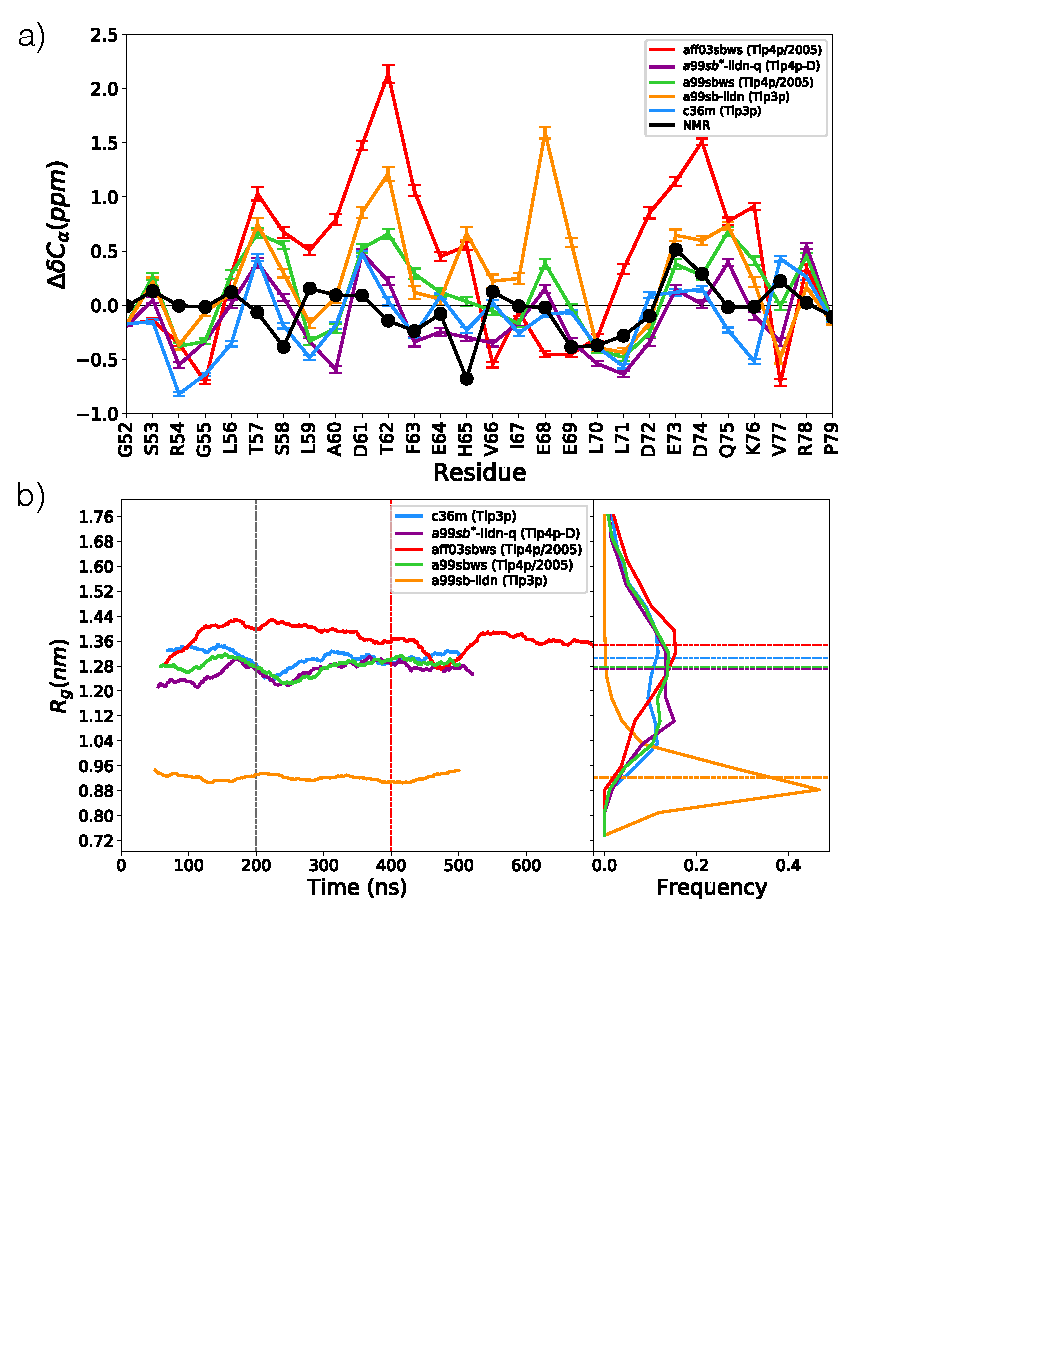
\includegraphics[scale=0.5,width=0.9\textwidth,trim={0 0cm 0 0cm},clip]{./figures/S1.pdf}
\caption{{\bf Force field comparison.} We ran T-REMD simulations of a 30 residue fragment of the V66 prodomain with several commonly used force field and water model combinations. (a) Comparison of $\Delta$$\delta$C\textsubscript{$\alpha$} secondary chemical shifts at 280K from MD ensembles for a99sb*-ildn-q~\cite {Lindorff-Larsen2010a, Hornak2006a} with Tip4p-D~\cite{Piana2015},  c36m ~\cite{Huang2016a}, a99sbws~\cite{Lindorff-Larsen2010a, Best2014}, a03sbws~\cite {Best2009, Best2014}, a99sb-ildn with Tip3p ~\cite {Jorgensen1981}, calculated using SPARTA+~\cite{Shen2010} and NMR from Ref.~\citenum{Anastasia2013}. (b) R\textsubscript{g} vs the simulation time, using a 100 ns moving window on left and R\textsubscript{g} distribution for each force field on right. Tip3p and a03sbws generates most collapsed and expanded R\textsubscript{g} distribution respectively. The equilibration time and $\langle R\textsubscript{g} \rangle$ is shown with vertical and horizontal dashed lines for each force field.}
\label{S1} 
\end{figure}

\begin{table}[!ht]
\centering
\caption{Summary of force field comparison simulations.}
\label{table2}
\begin{tabular}{|c|c|c|c|c|}  
\hline 
Force field & $\Delta$$\delta$C\textsubscript{$\alpha$} &  $\langle R_{\mathrm{g}} \rangle$  & equilibration time & no of replica\\
\hline
aff03sbws (Tip4p/2005) & 0.855 &  1.347 $\pm{0.007}$ & 400 ns & 36\\
\hline
a99sb*-ildn-q (Tip4p-D) & 0.355 &  1.270 $\pm{0.007}$ & 200 ns & 36\\
\hline
a99sbws (Tip4p/2005) & 0.425 &  1.277 $\pm{0.007}$ & 200 ns & 36\\
\hline
c36m (Tip3p)  & 0.350 &  1.306 $\pm{0.007}$ & 200 ns & 30\\
\hline
a99sb-ildn (Tip3p)  & 0.617 &  0.922 $\pm{0.003}$ & 200 ns & 32\\
\hline
\end{tabular}
\end{table}

\begin{figure}[!ht]
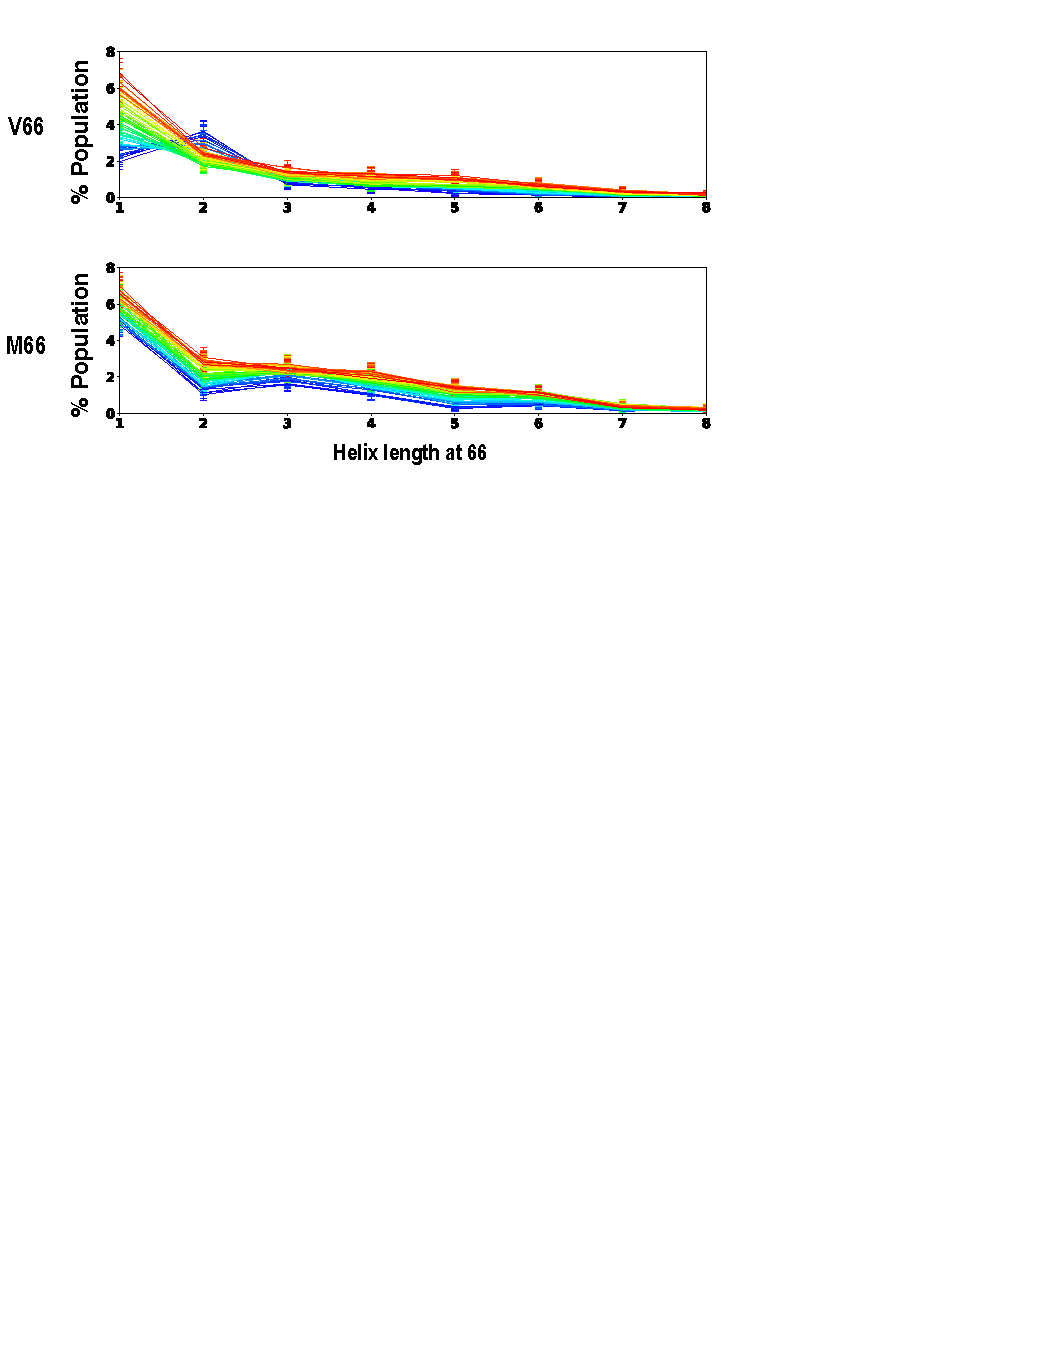
\includegraphics[scale=0.5,width=0.9\textwidth,trim={0 0cm 0 0cm},clip]{./figures/S2.pdf}
\caption{{\bf Effects of temperature and Val66Met mutation on helix propensity around residue 66.} Frequency of helix of a given length at residue 66 in V66 (top) and M66 (bottom) in the temperature range of 300K to 385 K. With the increase in temperature the color transitions from cooler (blue) to hotter (red).  It is entropically unfavorable for V66 and its neighboring residue to be simultaneously in the helical region of the Ramachandran map, as indicated by the decreasing helical propensity with increasing temperature.  For longer helices, the trend will depend more on the additional side-chains in the helix, and the trend with temperature is reversed, but it remains weaker than the analogous trend for the M66 sequence.  Errors represent standard error of a Bernoulli trial with n number of samples, where n is the product of total number unique replicas forming the helix of given length at residue 66 at a given temperature and average number of roundtrips per replica, 17.}
\label{S2} 
\end{figure}

\subsection{Heterogeneous behavior of individual domains}

\begin{figure}[!ht]
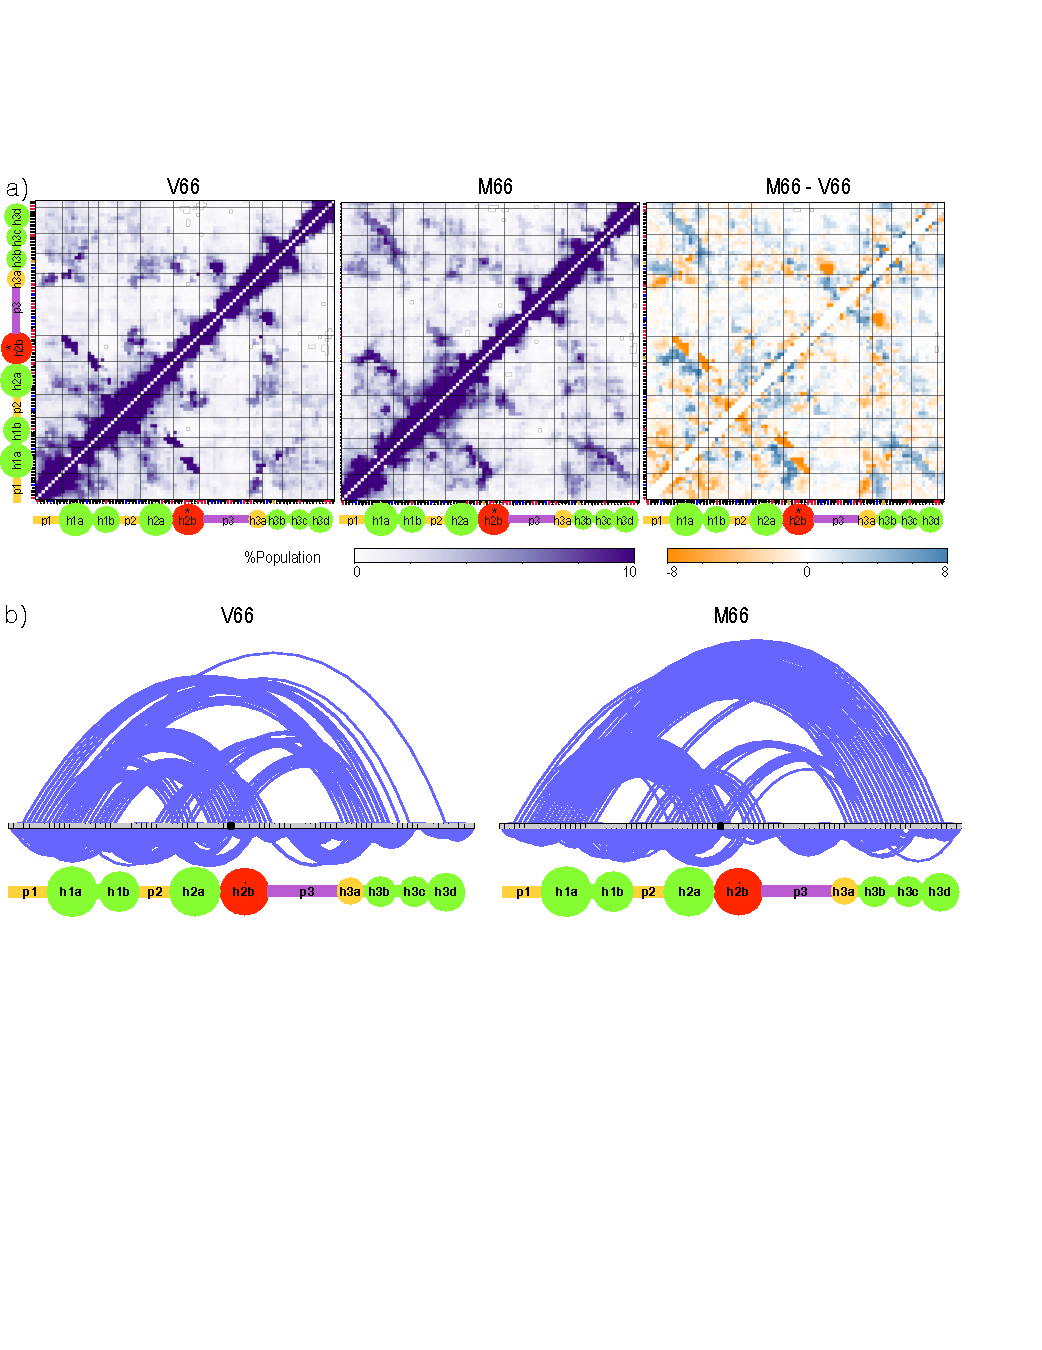
\includegraphics[scale=0.5,width=\textwidth,trim={0 0cm 0 0cm},clip]{./figures/S3.pdf}
\caption{{\bf Scaling behavior of each identified domain.} Ensemble averaged interchain distance profiles for the entire V66 and M66 prodomain and each blob in the sequence. 
Theoretical polymer scaling limits are shown with grey lines (prefactor A = 0.59 nm) (top). Flory exponents for each blob (bottom).}
\label{S2} 
\end{figure}

Disordered proteins can be well-described by Flory scaling theory $\langle R_{|i-j|}\rangle = A|i-j|^{\nu}$, where $\langle R_{|i-j|}\rangle$ is the ensemble-averaged internal distance, $|$i-j$|$ is residue separation along the chain, and $\nu$ is the Flory scaling coefficient\cite{Flory1949}. Larger values of $\nu$ correspond to swollen coils, while smaller values correspond to compact globules\cite{Das2013a}. In particular, when $\nu$=0.6 (``good solvent") the protein maximizes its interaction with solvent, and for $\nu$=0.33 (``poor solvent"), the protein maximizes self-interactions. The special intermediate case of $\nu$=0.5 is called a ``theta solvent"\cite{Flory1949}. Most IDPs that obey this scaling behavior have $\nu$$>$0.5\cite{Hofmann2012,Das2013a,Zerze2015,Meng2018}. 

As shown in Fig~\ref{S2} the prodomain as a whole is not well fit by a single power law: for separations of 15 or fewer residues the prodomain falls in the ``theta solvent" regime, while for separations of 20 or more residues it falls in the ``poor solvent" regime. Each identified individual domain does obey a power law, and we calculated A and $\nu$ for each domain as if it was isolated from rest of the protein (Fig~\ref{S2}). The highest observed value of $\nu$ was in h2b and h3c domain. This is in agreement with strong polyelectrolyte nature of h2b and high content of Proline residue (20\%)  in h3c.



\textbf{Method} We calculated the average distance between the first atom (N) and last atom (O) for all residue pairs of a given sequence as a function of sequence separation $|i-j|$ using $g_{-}traj$. 
Errors before fitting were calculated as the standard error in the mean, where $n =  1088$ is the product of total number of replicas simulated (64) and average number of roundtrips per replica (17).   $\nu$ was calculated by linear fit of ln($\langle R_{|i-j|}\rangle)$ vs $ln(|i-j|)$
weighted by each point's pre fit error with fixed A of 0.59nm. To exclude the short-range backbone rigidity, distances with $|i-j|$ $<$ 3 were not fit.

% For domain h2 the value of $\nu$ ($\nu$=0.42 $\pm { 0.1}$), is most compact among all three hydrophobic domains, and lies between poor and theta solvent. For p3, $\nu$= 0.63 $\pm { 0.1}$, reaches the good solvent limit, which is consistent with the low hydrophobicity and expanded (excluded volume limit) coil conformations as predicted from phase behavior of a strong polyampholyte with low $\kappa$~\cite {Das2013a} (Table~\ref{table2}). 



\begin{figure}[!ht]
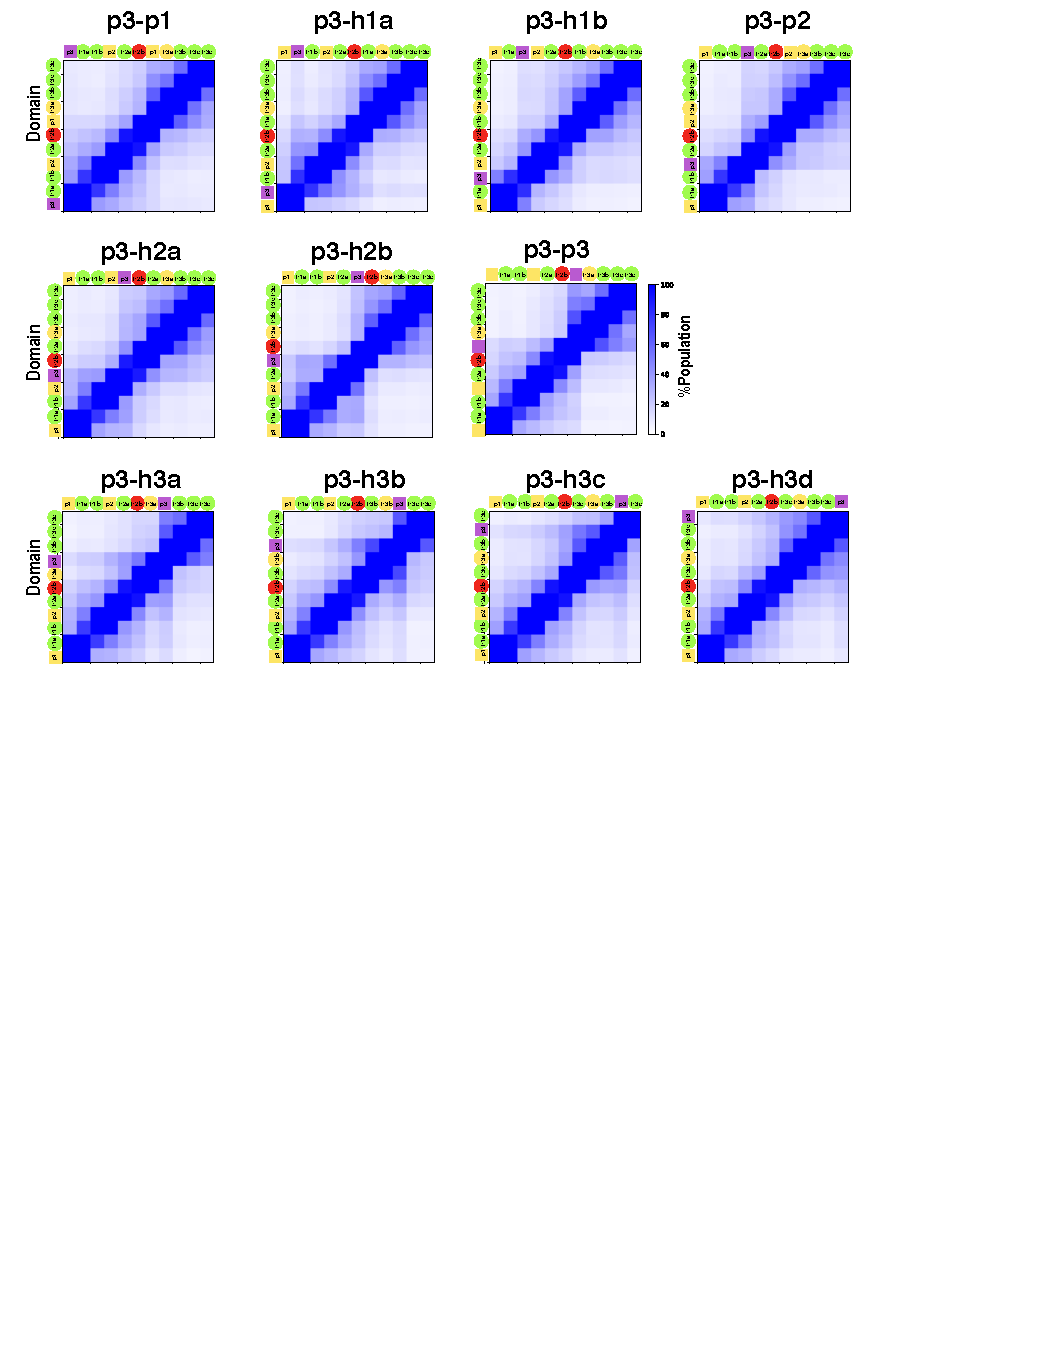
\includegraphics[scale=0.5,width=\textwidth,trim={0 0cm 0 0cm},clip]{./figures/S4.pdf}
\caption{{\bf Effect of perturbing monomer properties on freely-jointed, self-avoiding heteropolymer} Contact probability maps from MC simulations, analogous to those in Figure 5a of the main text, in which the blob p3 is swapped with every other blob in the chain, with the new location represented by the purple square in the graph annotation.  As the p3 blob is shifted along the chain, p3 and p1 consistently bound a white ``forbidden'' region that has little interaction with the rest of the protein. }
\label{S4} 
\end{figure}

\begin{figure}[!ht]
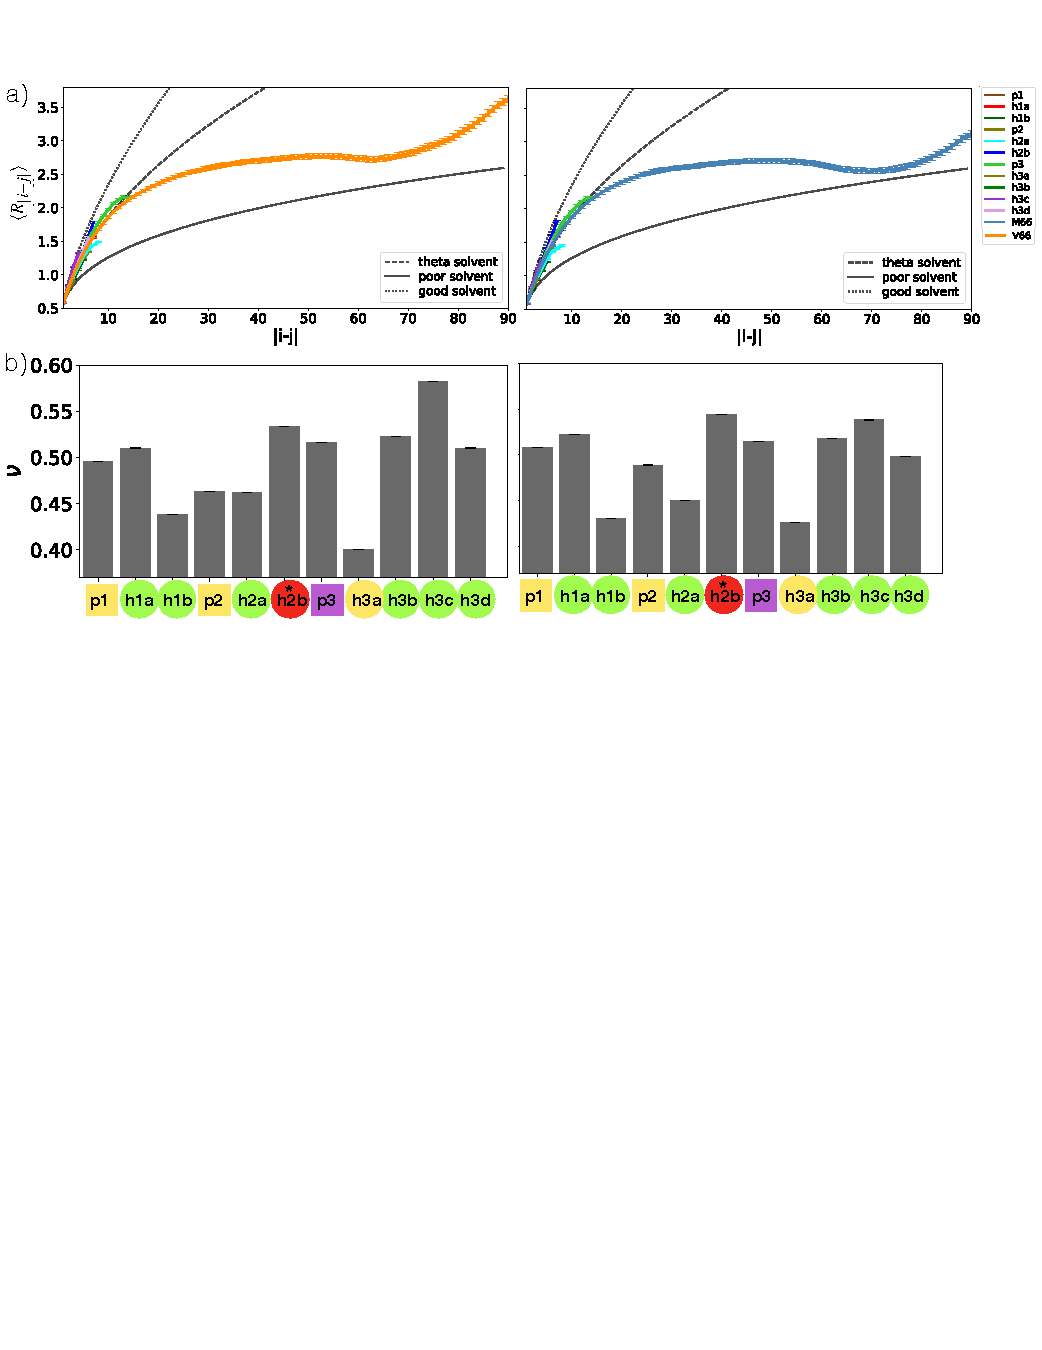
\includegraphics[scale=0.5,width=0.9\textwidth,trim={0 0cm 0 0cm},clip]{./figures/S5.pdf}
\caption{{\bf $\beta$-pairing of each blob pair} $\beta$ propensities at each residue in V66 sequence (top) and M66 sequence (bottom) for four clusters. Frames were first clustered by whether the X-Y contact was formed (purple) or broken (green), and then by whether $\beta$ structure was present in X (solid) or absent (dashed). X represents p1 and is annotated at the top panel and Y represents other blobs identified in the sequence and is annotated on the left for each panel. Errors represent standard error of a Bernoulli trial with n number of samples, where n is the product of total number of unique replicas in a given cluster and average number of roundtrips per replica (17).} 
\label{S9} 
\end{figure}

\begin{figure}[!ht]
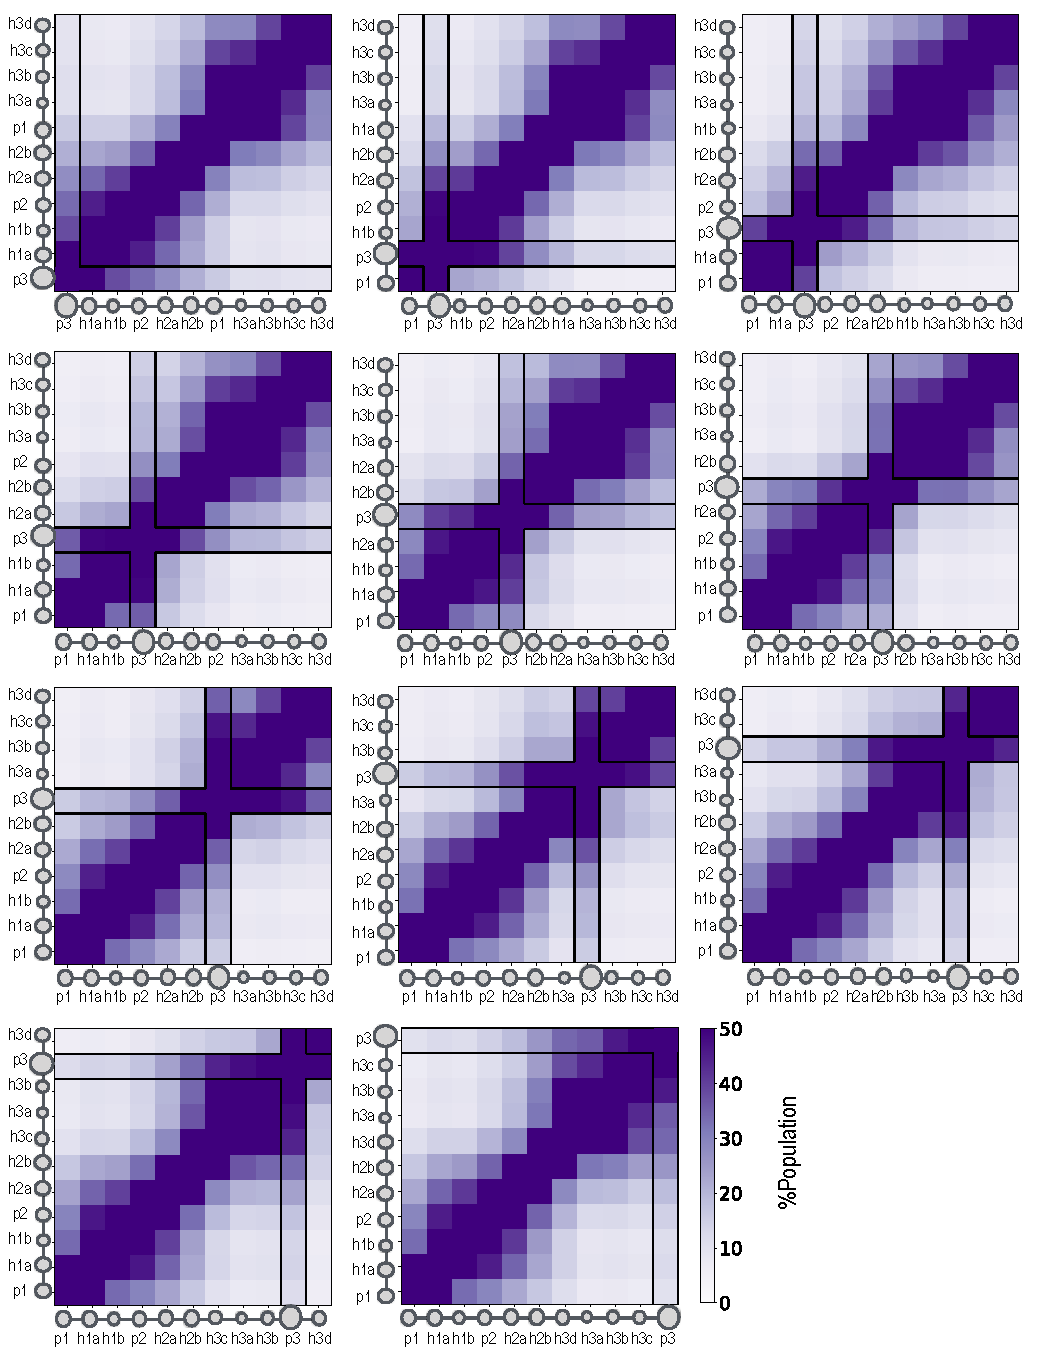
\includegraphics[scale=0.5,width=0.9\textwidth,trim={0 0cm 0 0cm},clip]{./figures/S6.pdf}
\caption{{\bf $\beta$-pairing of each blob pair.} Same as Fig S5, where X represents h1a (left) or h1b(right).} 
\label{S5} 
\end{figure}

\begin{figure}[!ht]
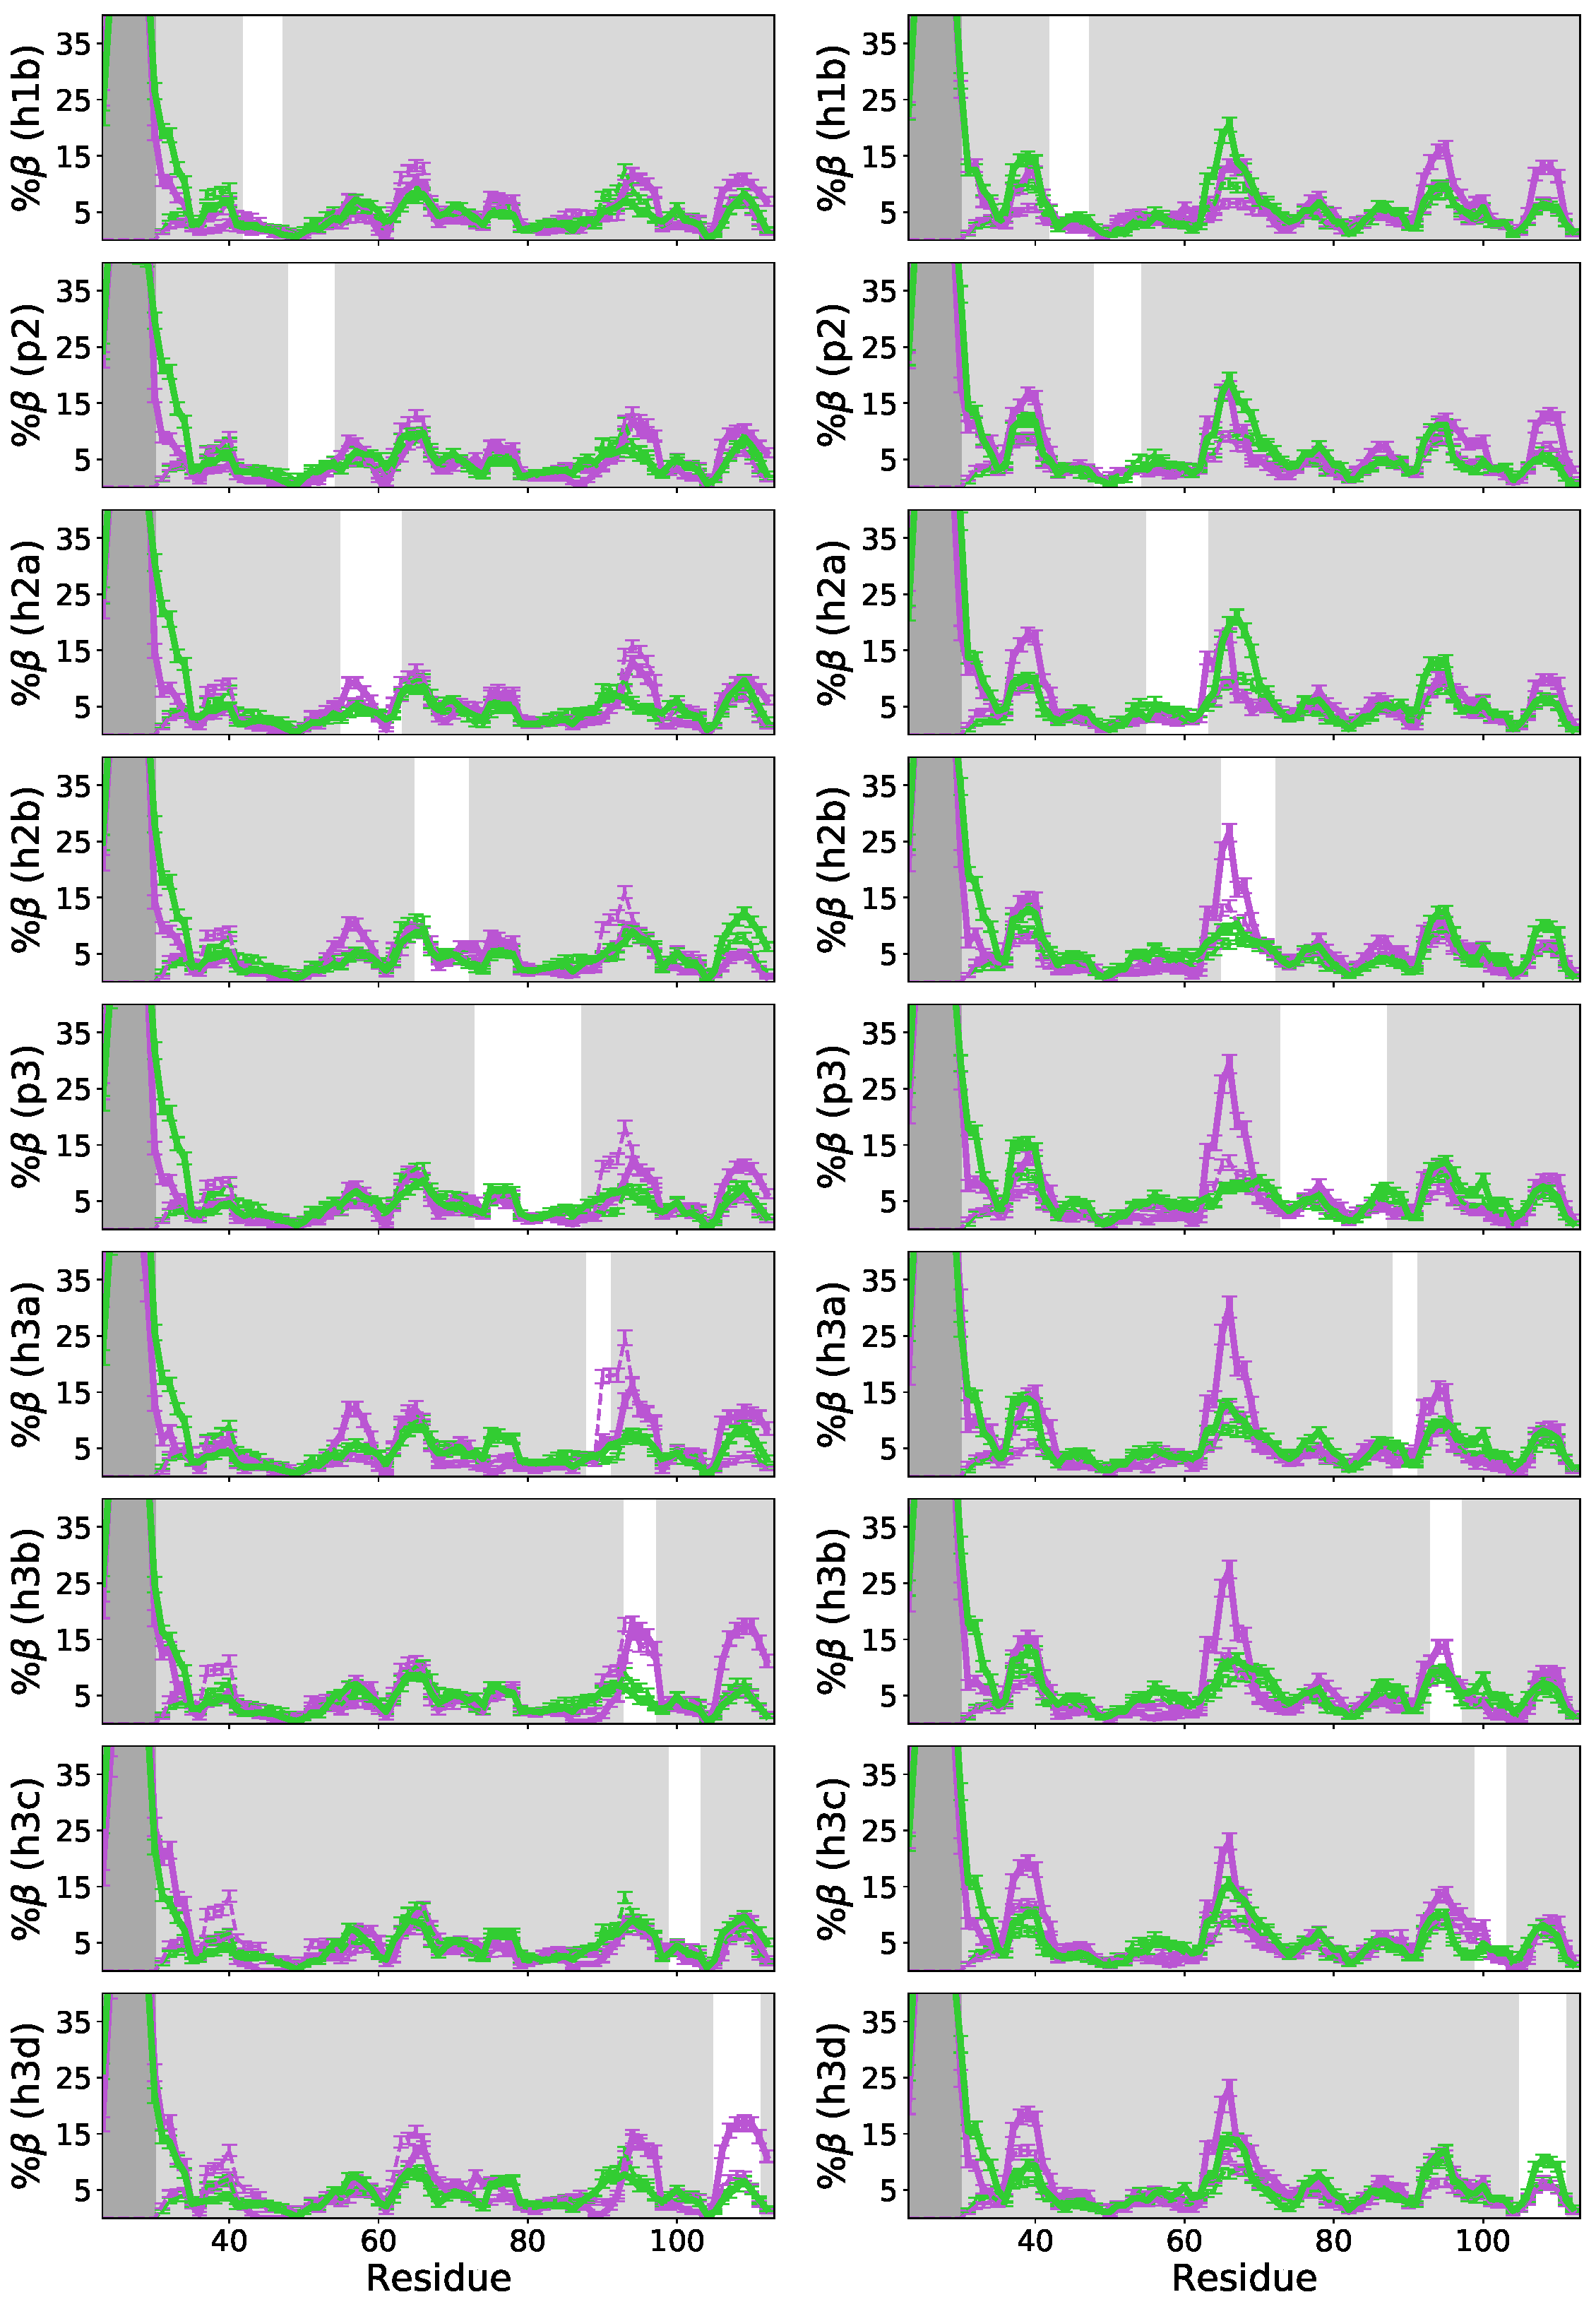
\includegraphics[scale=0.5,width=0.9\textwidth,trim={0 0cm 0 0cm},clip]{./figures/S7.pdf}
\caption{{\bf $\beta$-pairing of each blob pair.} Same as Fig S5, where X represents h2a (left) or h2b(right).} 
\label{S6} 
\end{figure}

\begin{figure}[!ht]
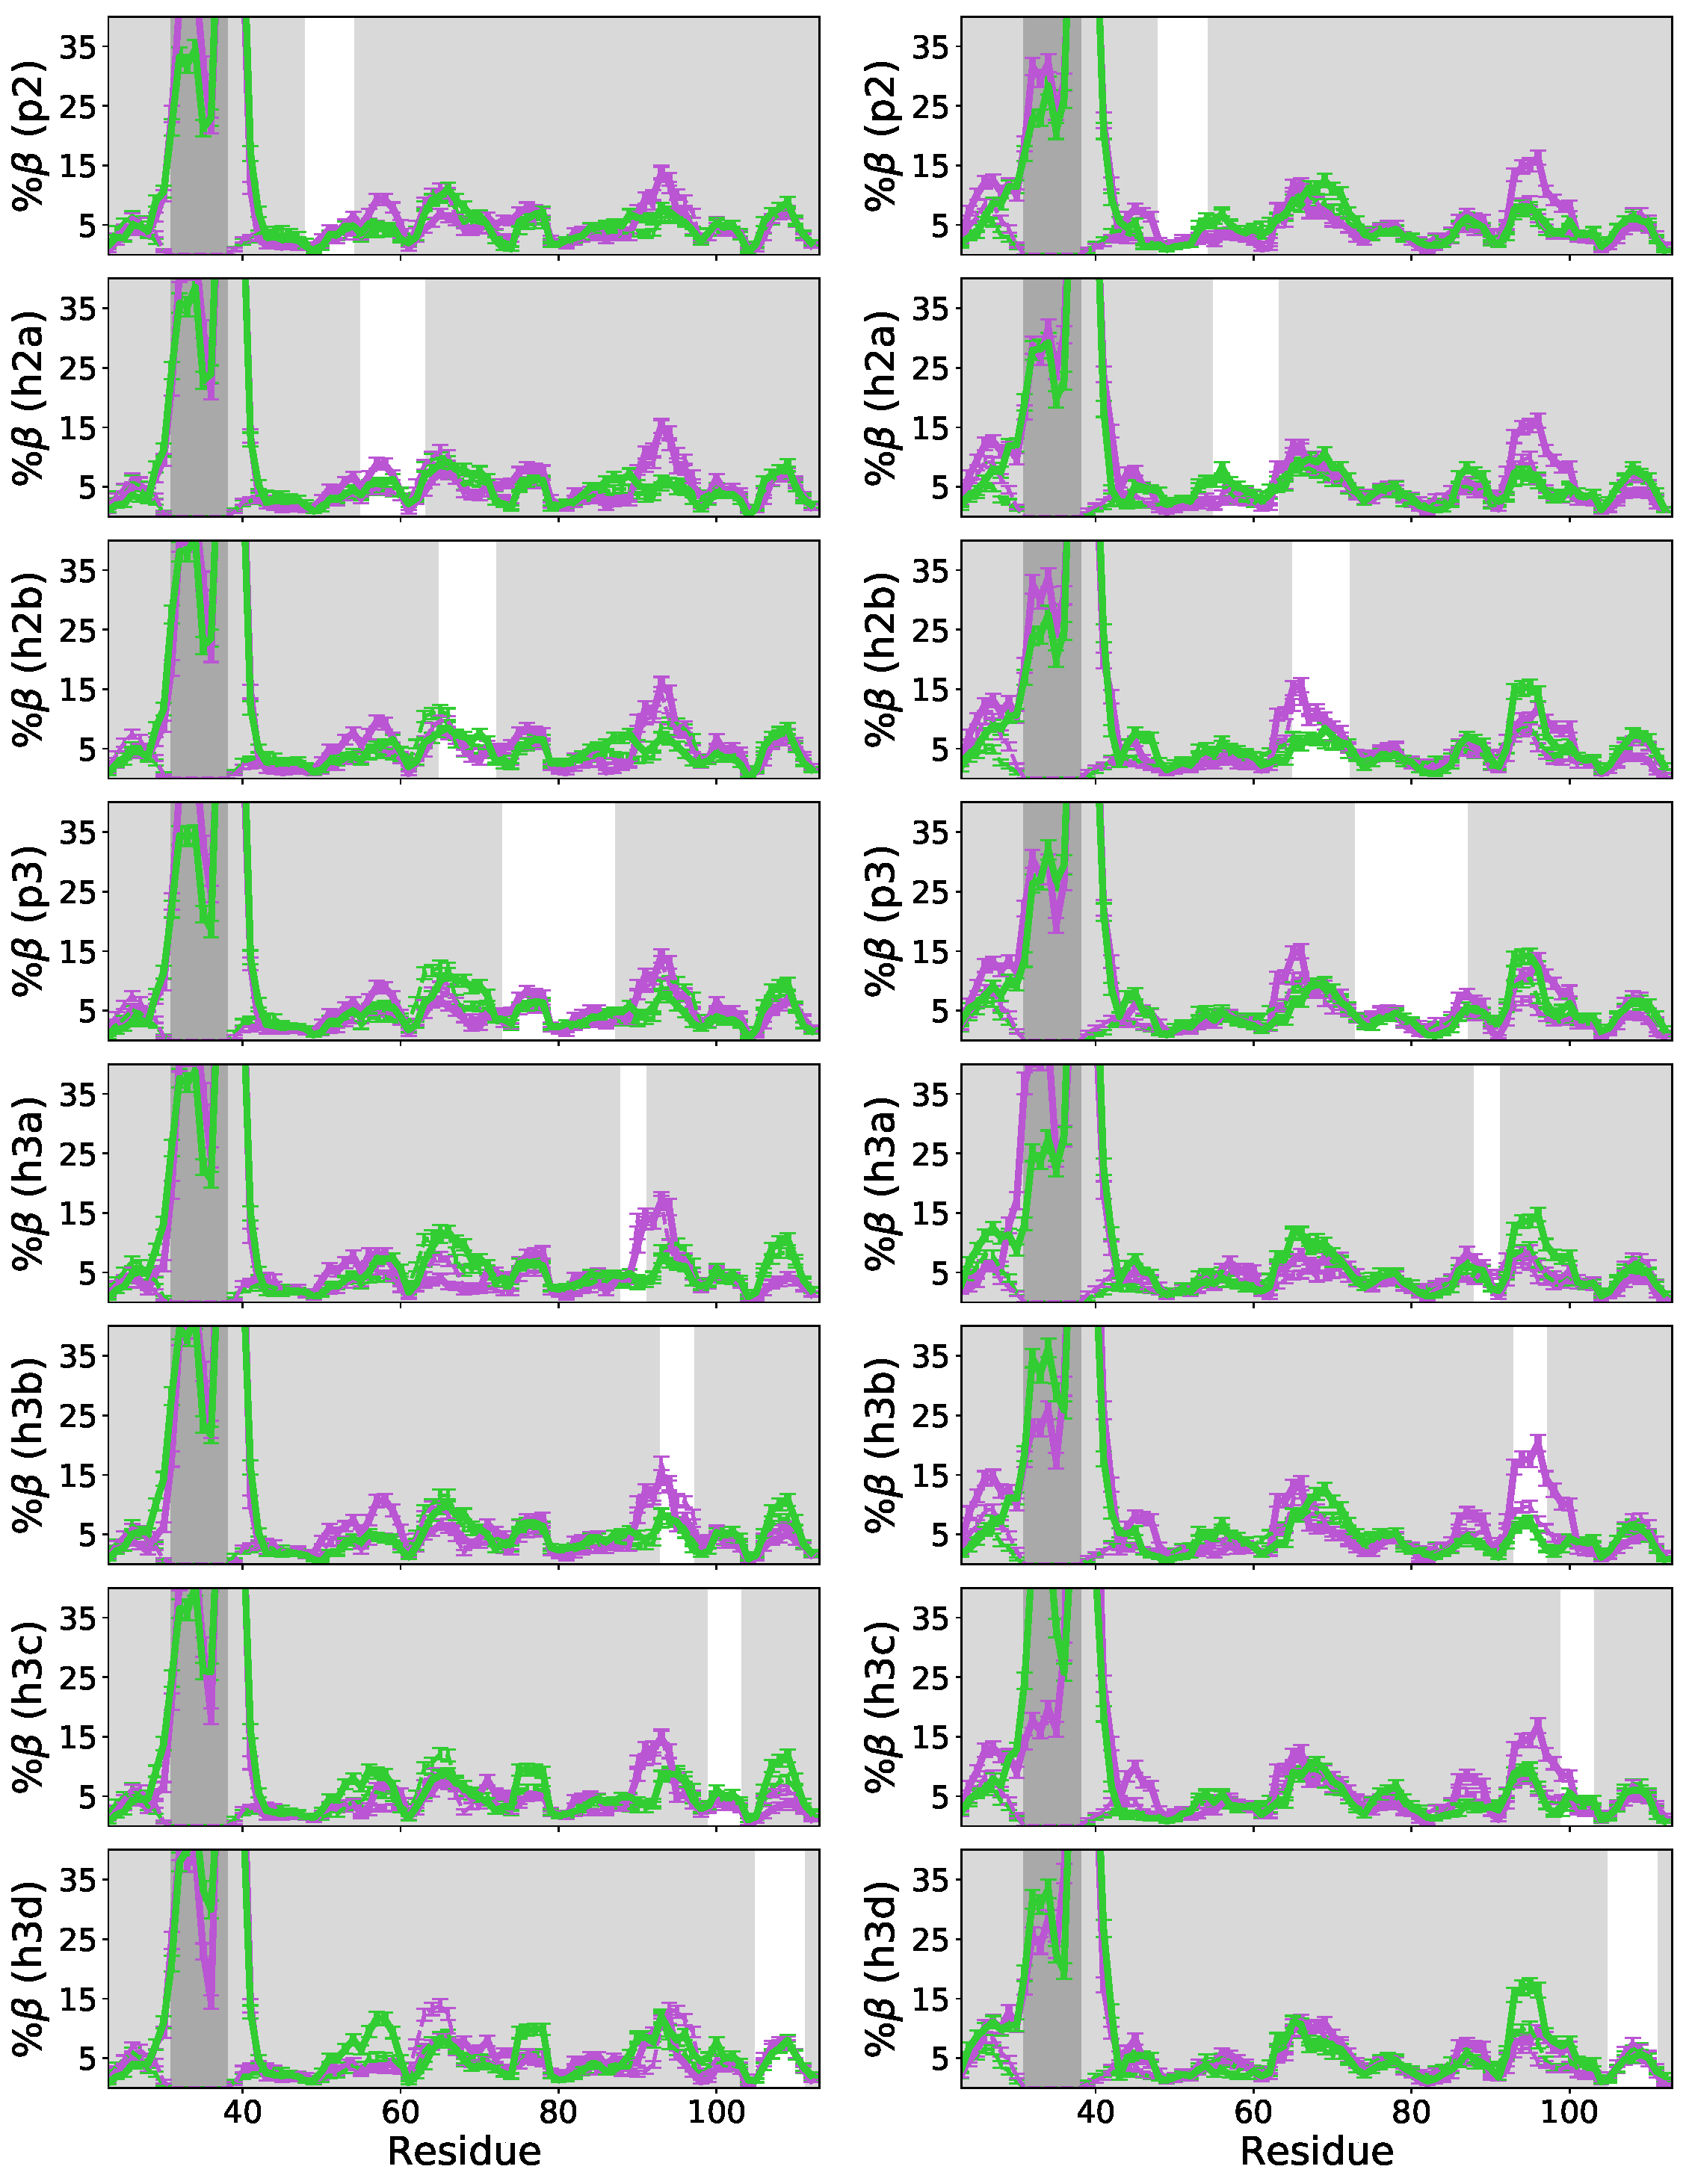
\includegraphics[scale=0.5,width=0.9\textwidth,trim={0 0cm 0 0cm},clip]{./figures/S8.pdf}
\caption{{\bf $\beta$-pairing of each blob pair.} Same as Fig S5, where X represents h3a (left) or h3b(right).} 
\label{S7} 
\end{figure}

\begin{figure}[!ht]
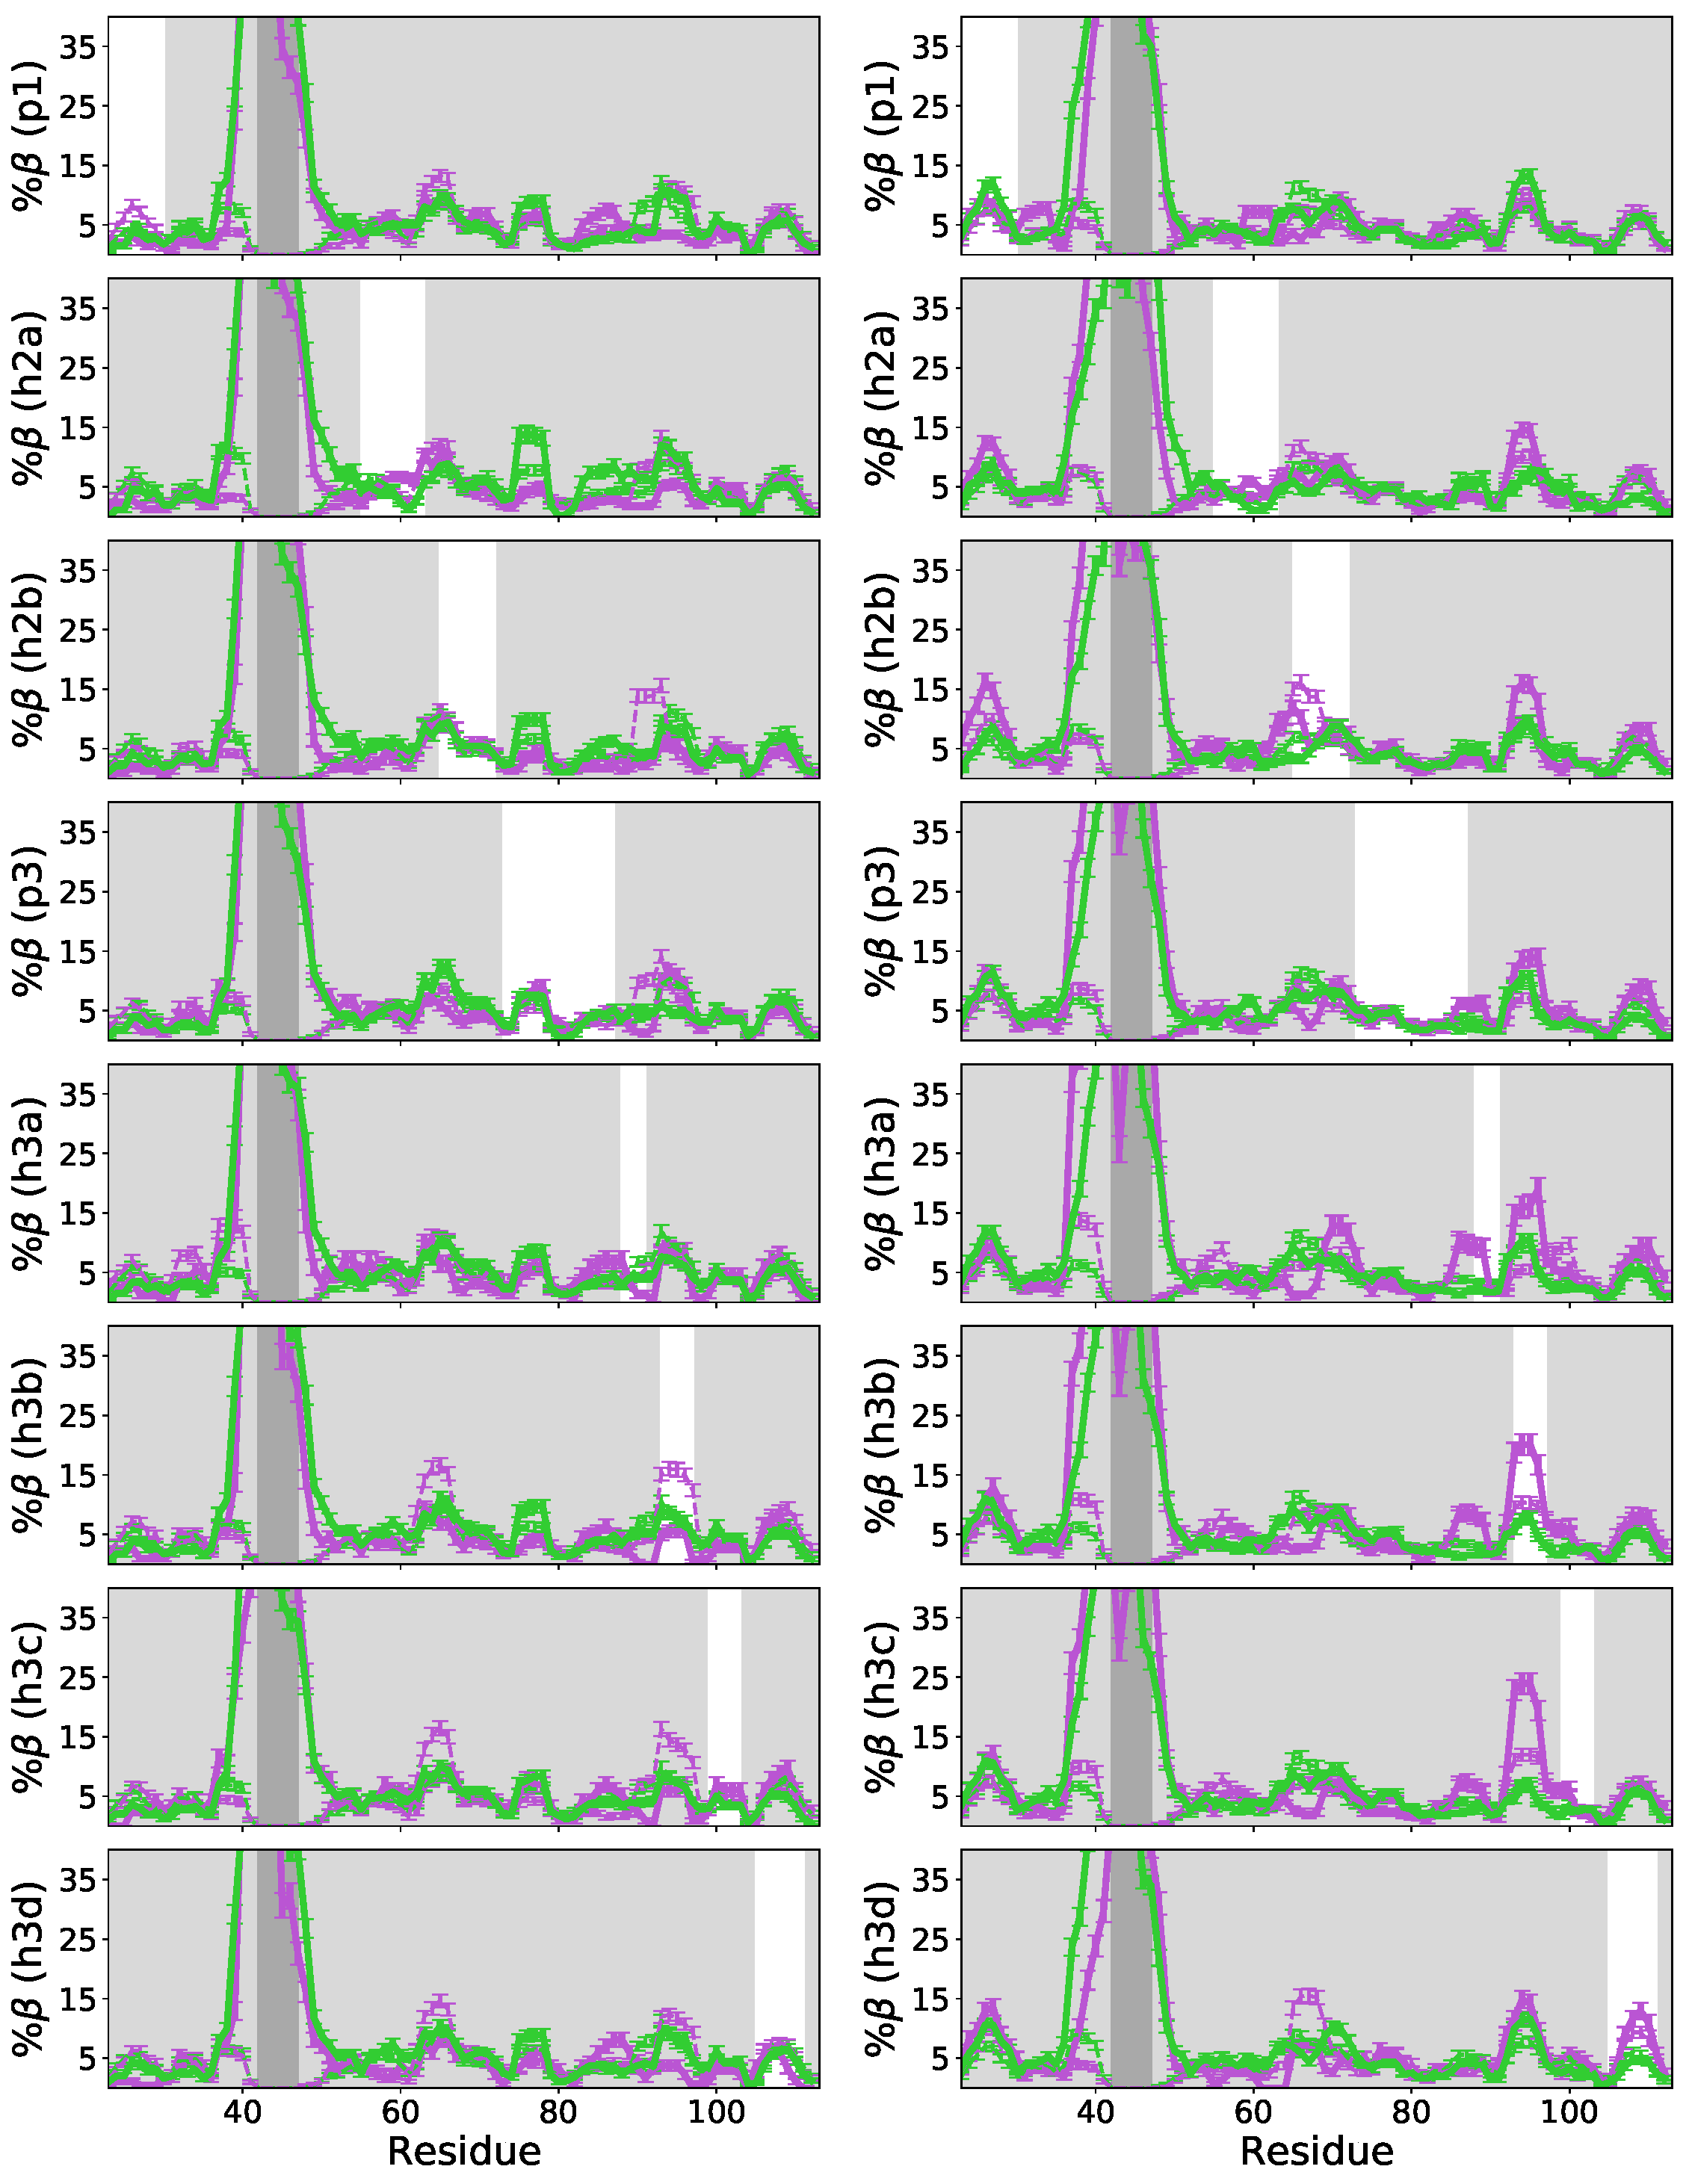
\includegraphics[scale=0.5,width=0.9\textwidth,trim={0 0cm 0 0cm},clip]{./figures/S9.pdf}
\caption{{\bf $\beta$-pairing of each blob pair.} Same as Fig S5, where X represents h3c (left) or h3d(right).} 
\label{S8} 
\end{figure}


\begin{figure}[!ht]
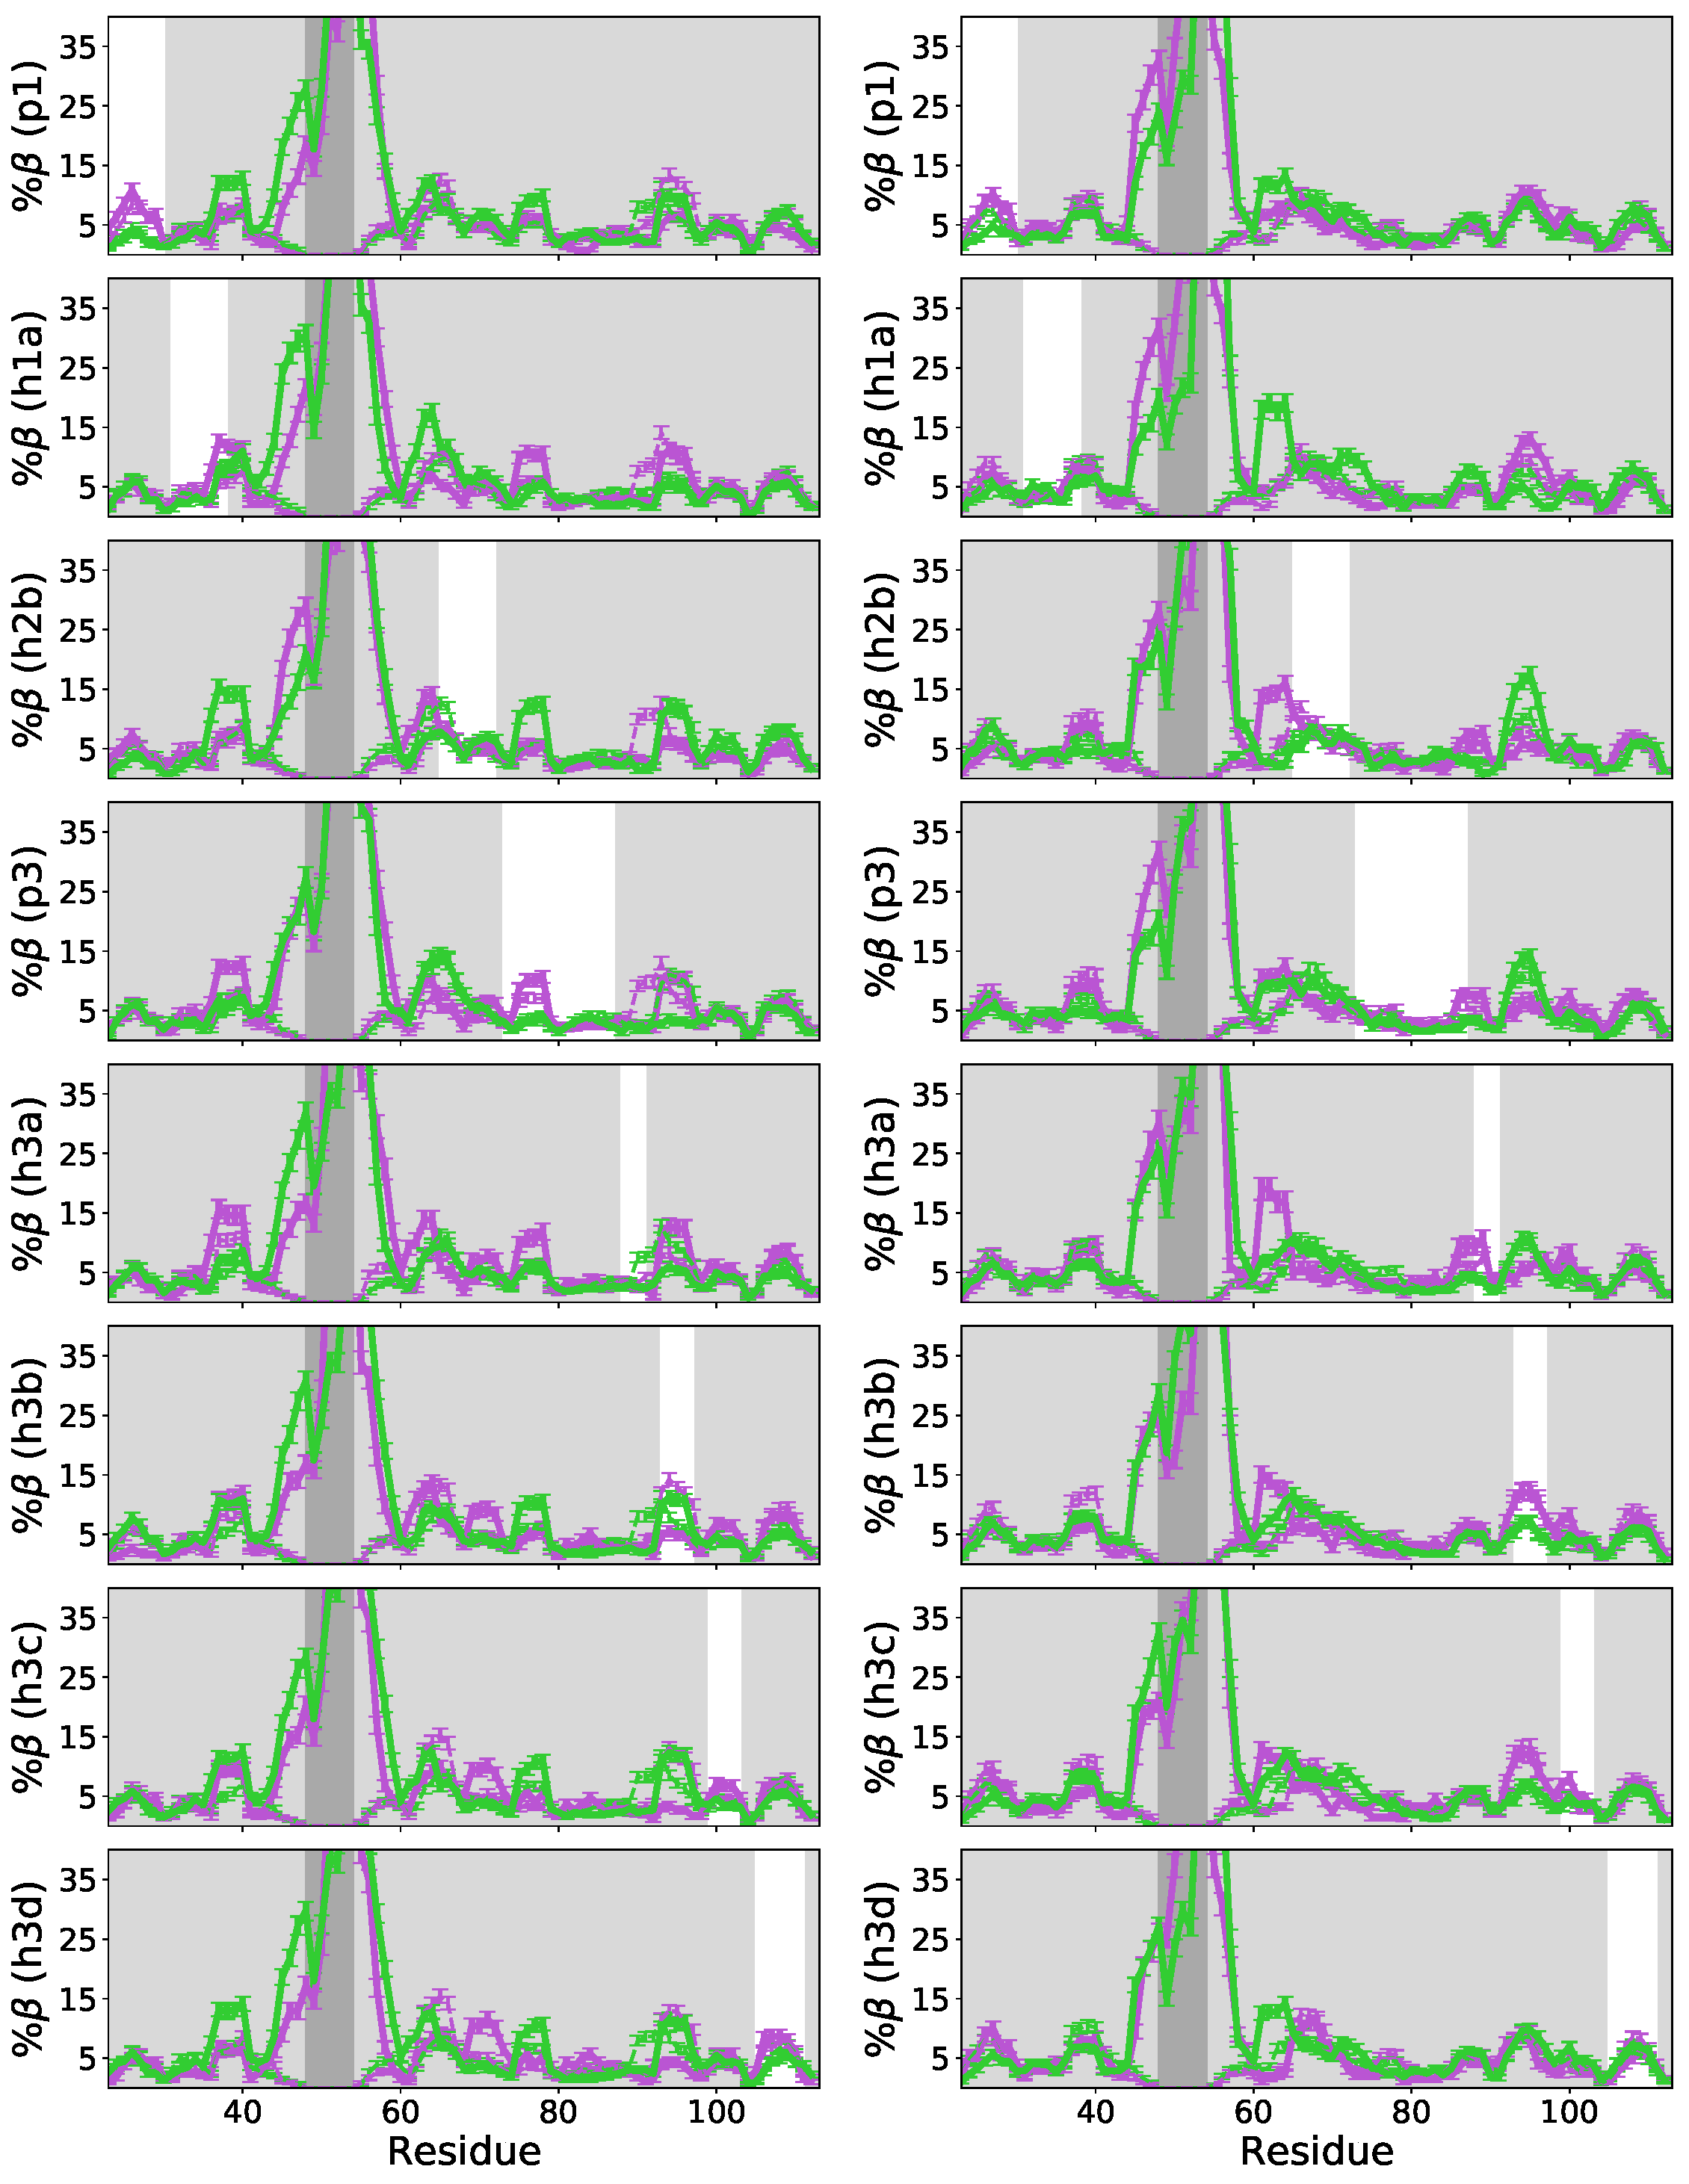
\includegraphics[scale=0.5,width=0.9\textwidth,trim={0 0cm 0 0cm},clip]{./figures/S10.pdf}
\caption{{\bf $\beta$-pairing of each blob pair.} Same as Fig S5, where X represents p2 (top) or p3 (bottom).} 
\label{S10} 
\end{figure}

\begin{figure}[!ht]
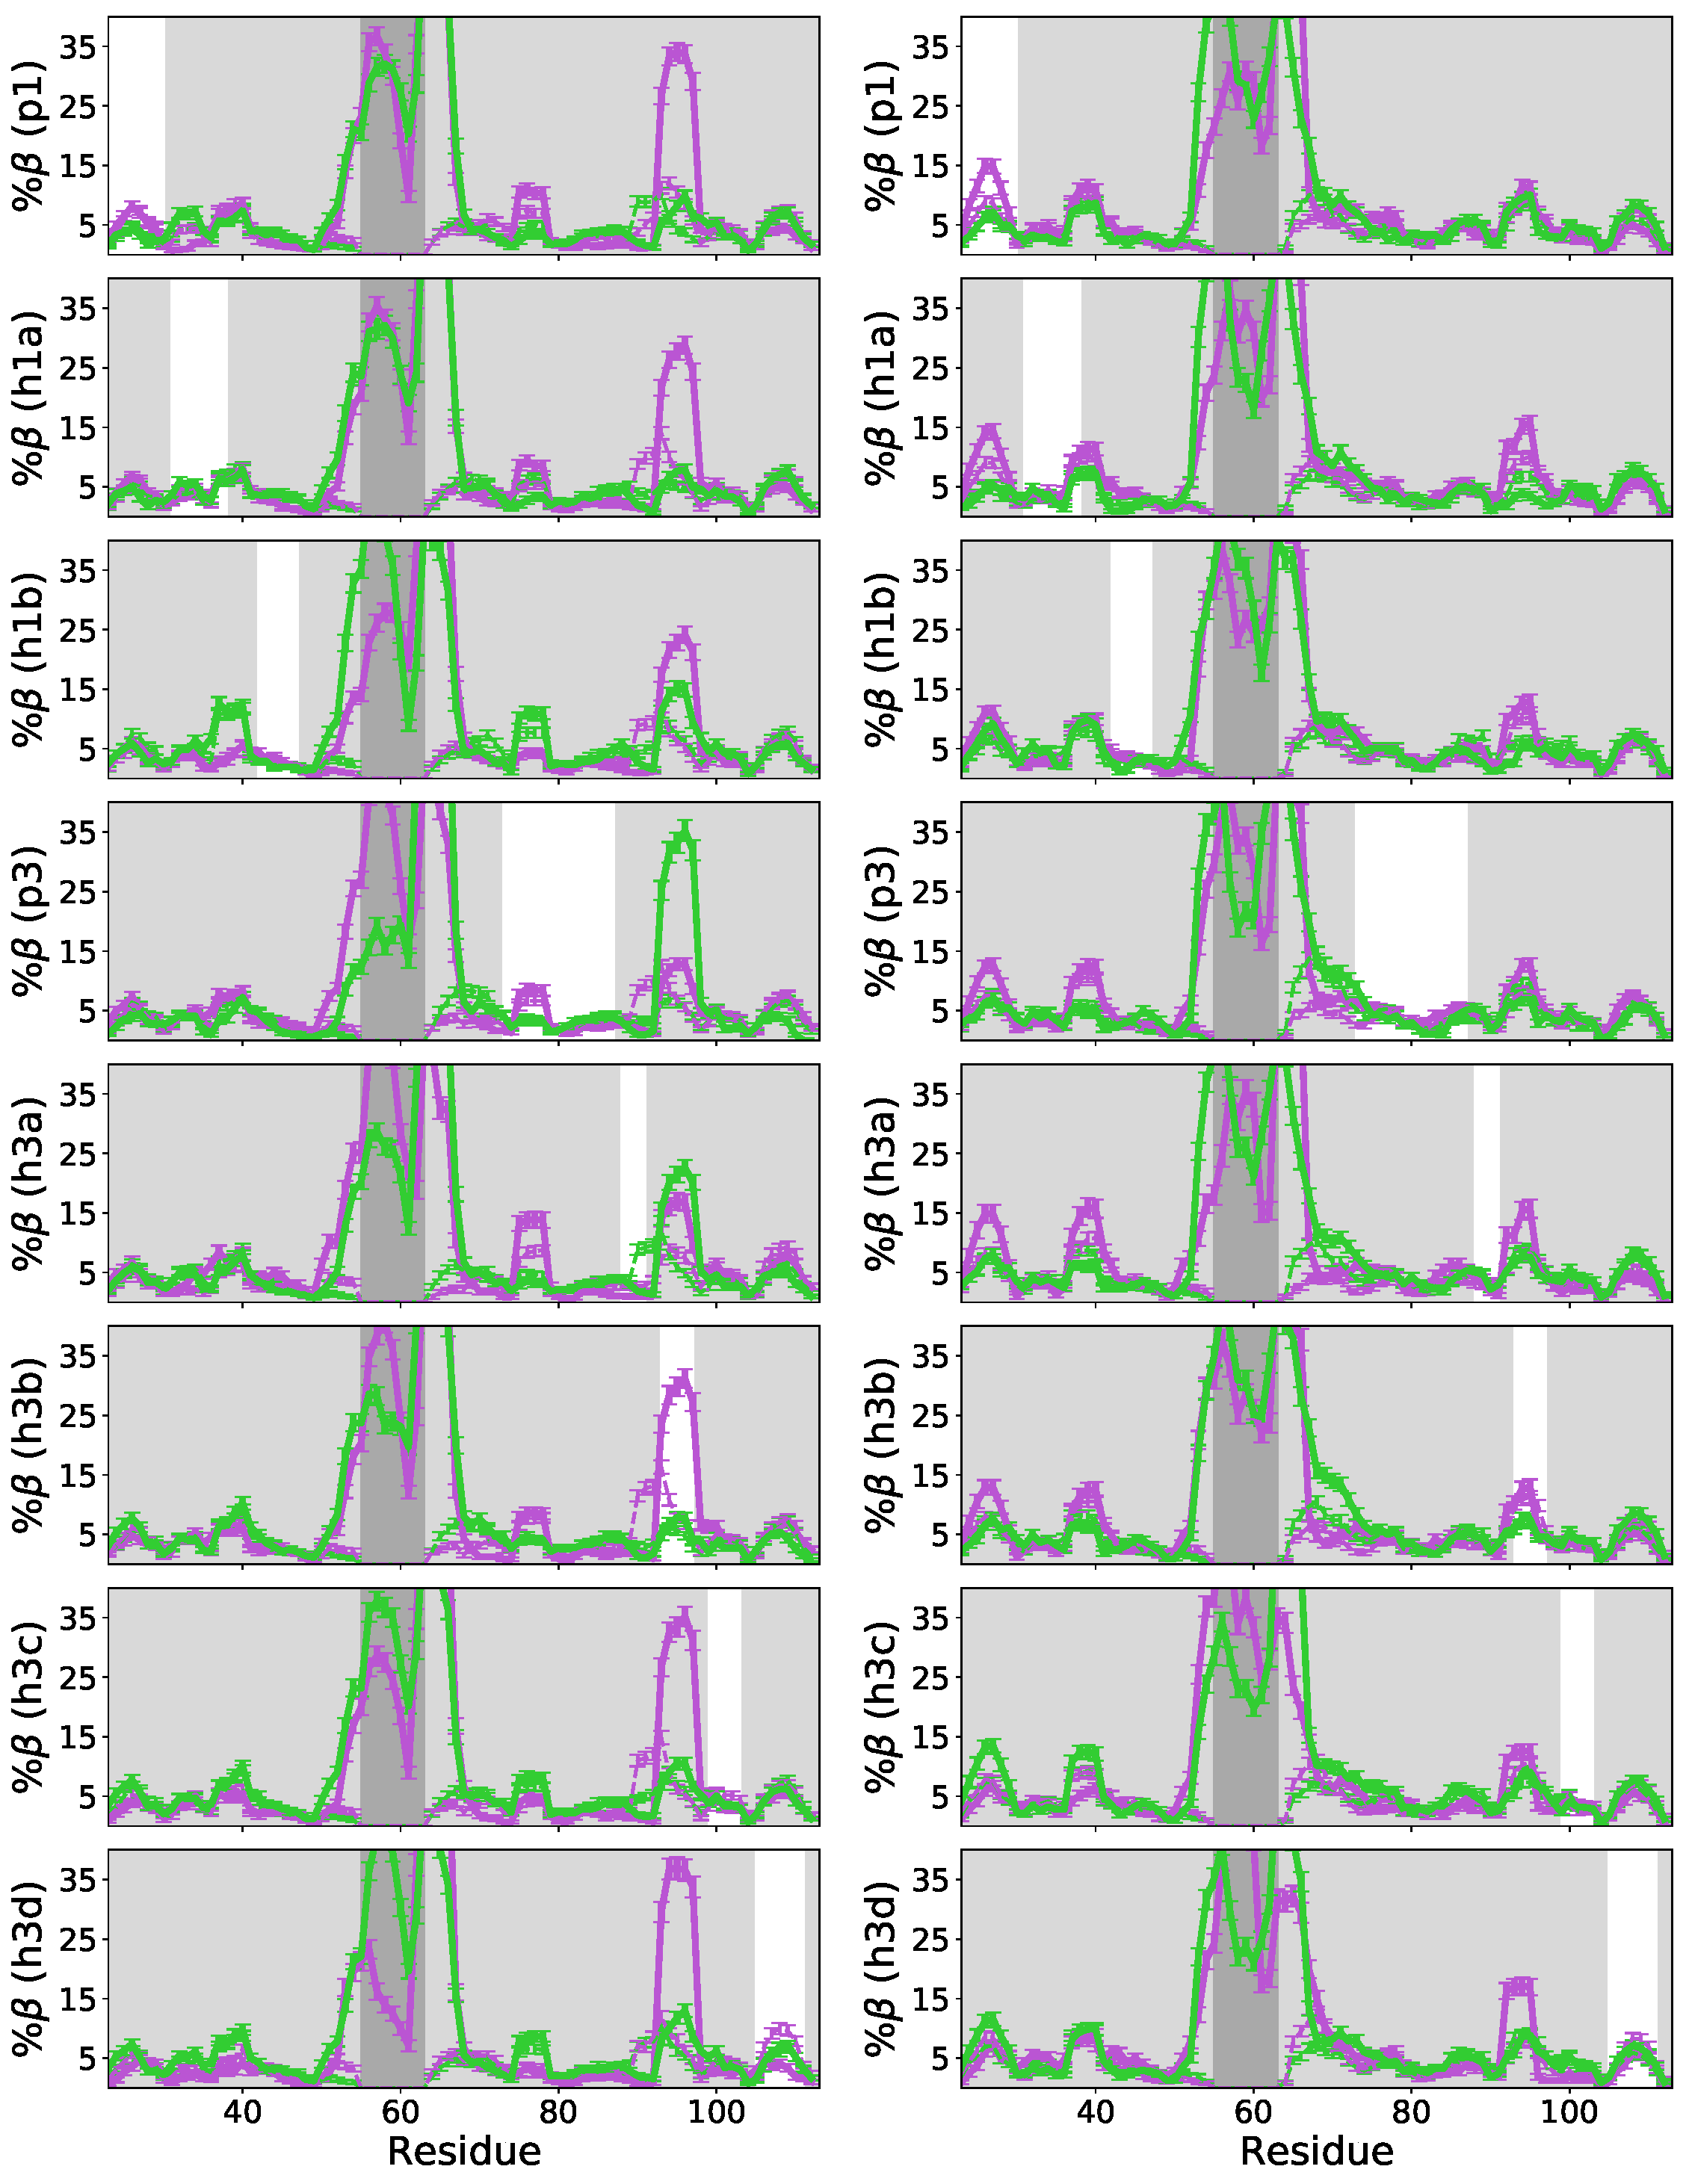
\includegraphics[scale=0.5,width=\textwidth,trim={0 0cm 0 0cm},clip]{./figures/S11.pdf}
\caption{{\bf Residue level contacts for the entire prodomain.} Contact probability between every residue pair for V66 (left) and M66 (middle) and M66-V66(right). Two residue pairs are in contact if the distance between C\textsubscript{$\alpha$}-C\textsubscript{$\alpha$} atoms between the two residues are 0.8nm or less. b)  A linear network of transient tertiary contacts shown in a). The contact networks were build using Cytoscape~\cite{Ahlstrom2013} with a linear representation of residues. Each protein residue comprises a node in the network, with interactions between residues represented as edges. The strength of individual interactions can be interpreted by the thickness of the edge line on the network diagram. If the separation between residues forming the contact is more than 3, its edge is drawn above the node; otherwise, the edge is drawn at the bottom of the node. To focus on significant interactions, interactions showing more than 4\% persistence were considered in network visualization.}
\label{S11} 
\end{figure}

\begin{figure}[!ht]
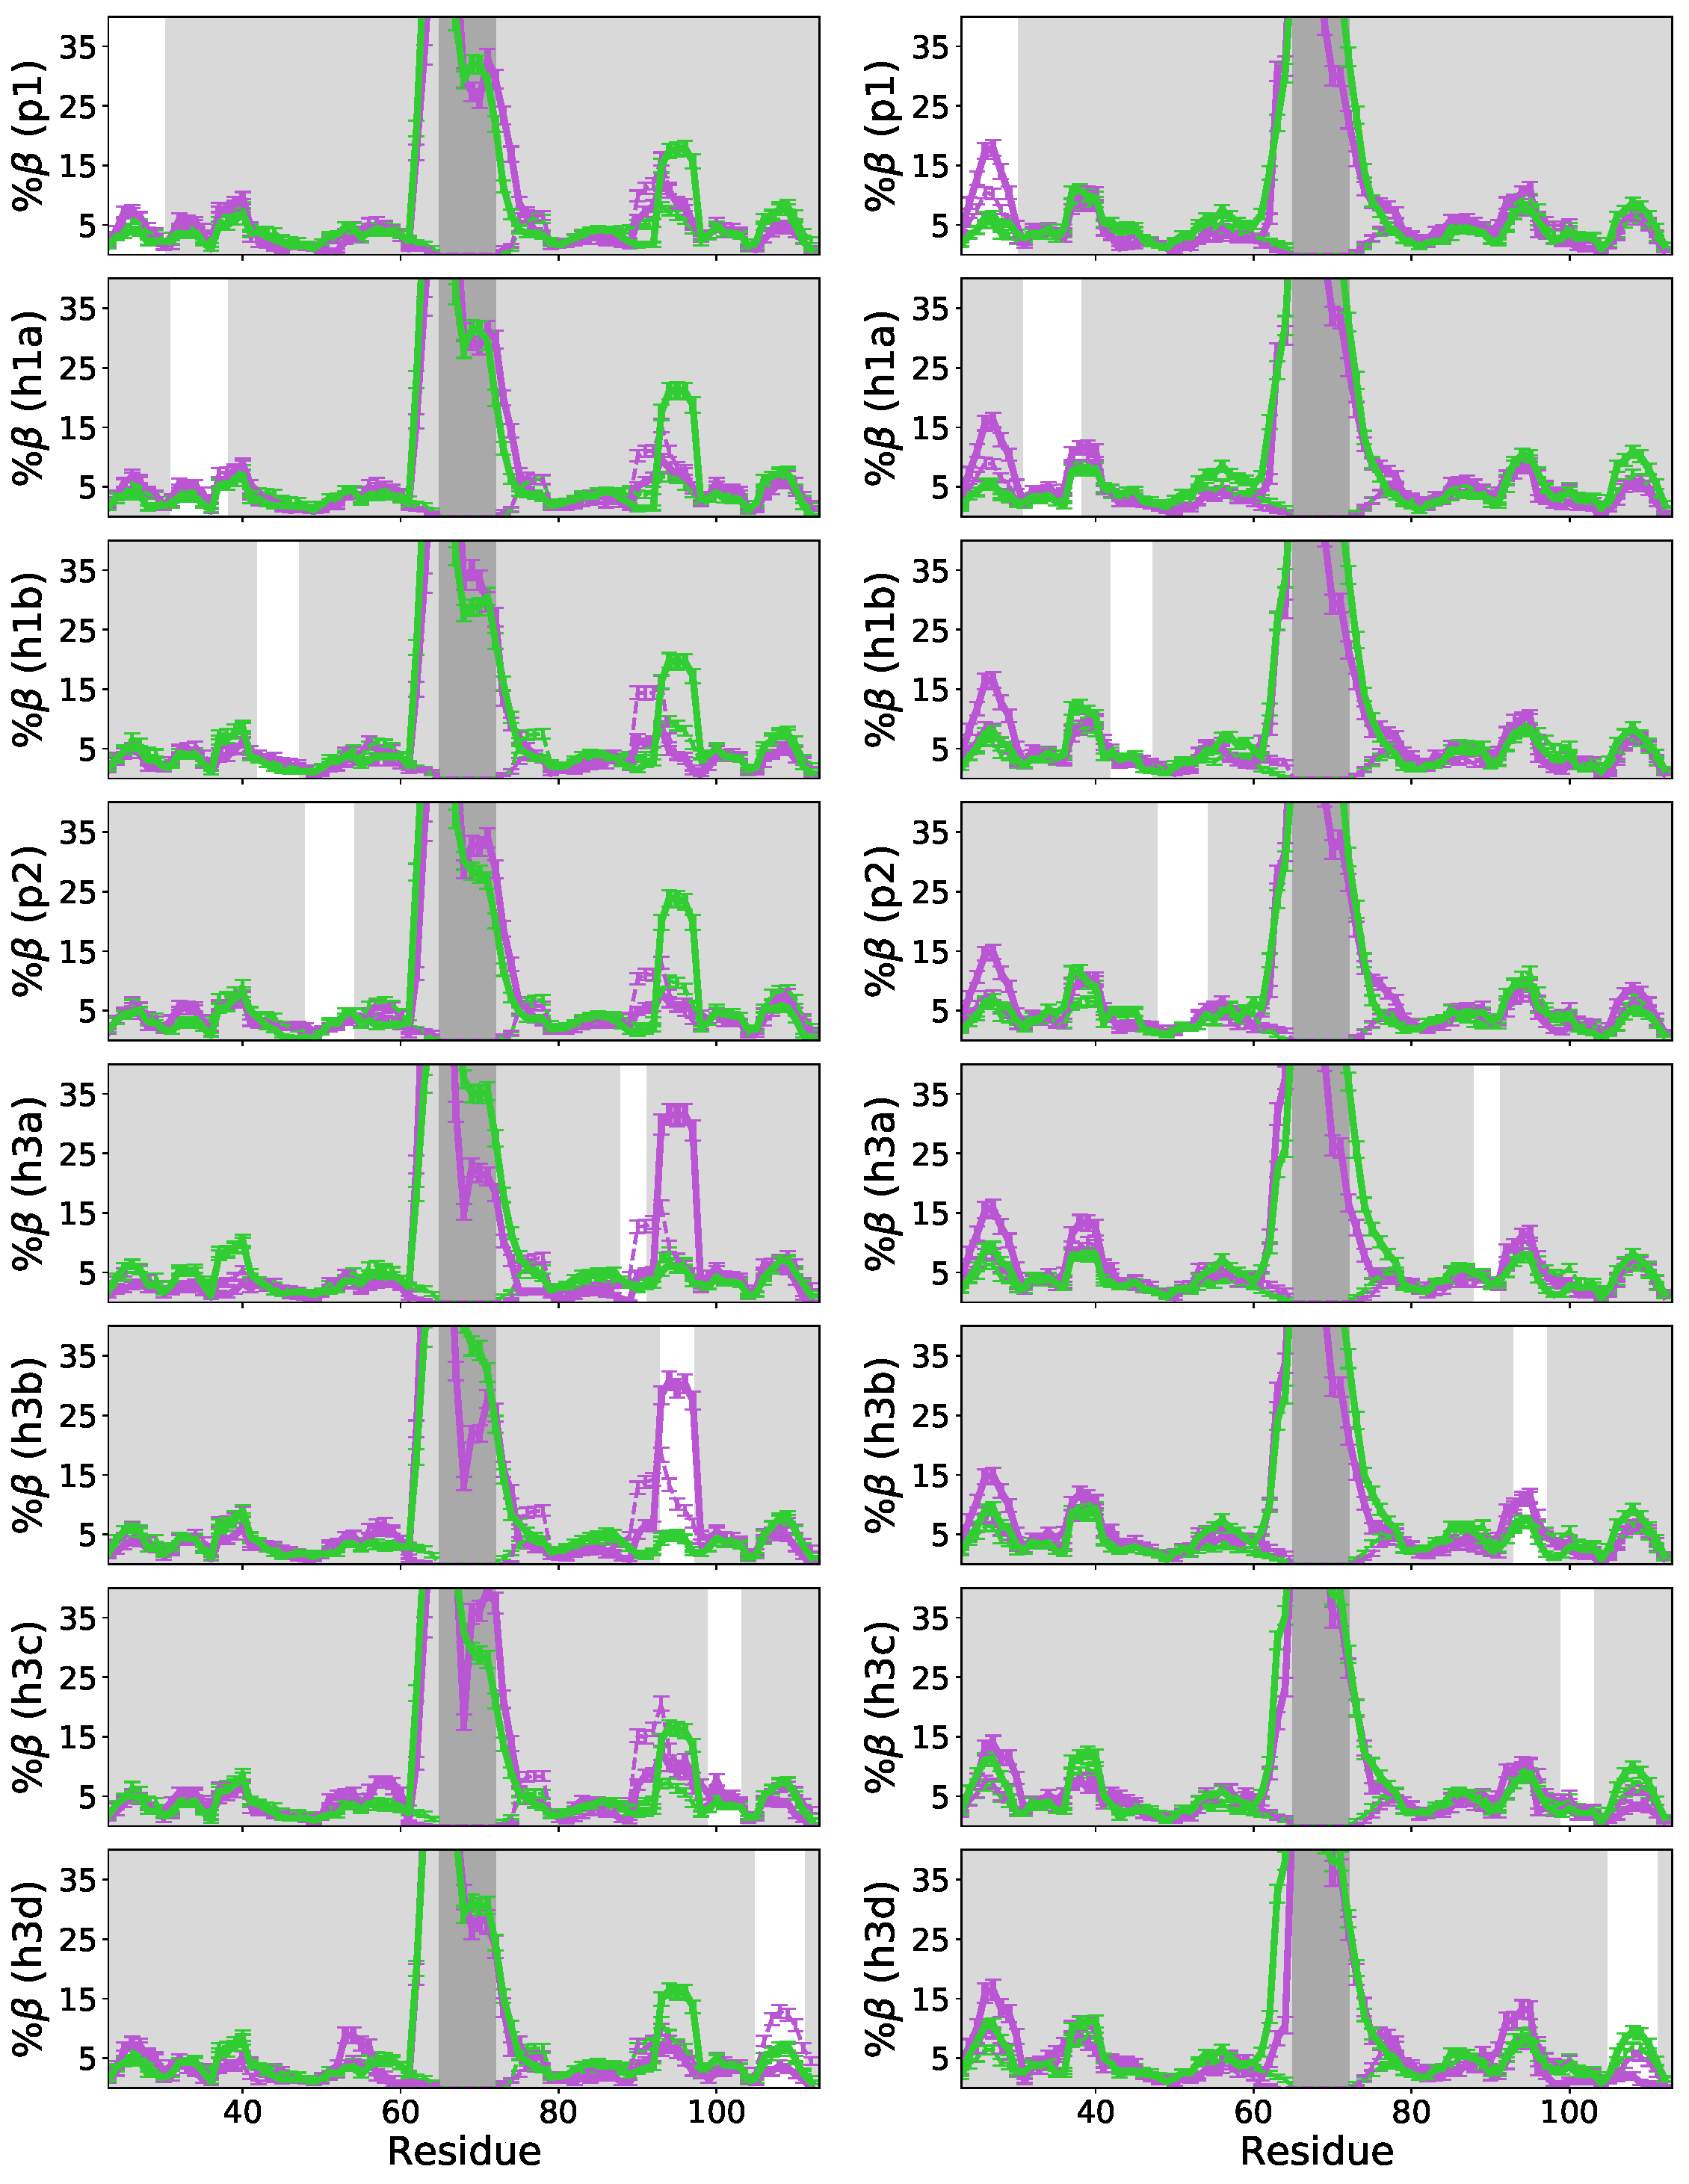
\includegraphics[scale=0.5,width=\textwidth,trim={0 0cm 0 0cm},clip]{./figures/S12.pdf}
\caption{{\bf Residue level contacts for the entire prodomain.} Contact probability between every residue pair for V66 (left) and M66 (middle) and M66-V66(right). Two residue pairs are in contact if the distance between backbone-backbone atoms between the two residues are 0.4nm or less (1st row), if the distance between non hydrogen sidechain-siechain atoms between the two residues are 0.4nm or less (2nd row), if the distance between non hydrogen sidechain-siechain atoms between the two hydrophobic residues are 0.4nm or less (3rd row), if the two residue pairs are forming a salt bridge with the distance between the donor and acceptor atoms $<$ 0.32nm (4th row).}
\label{S12} 
\end{figure}


\clearpage

\bibliography{IDP_Val66Met_Lohia}

\end{document}

